%%%%%%%%%%%%%%%%%%%%% chapter.tex %%%%%%%%%%%%%%%%%%%%%%%%%%%%%%%%%
%
% sample chapter
%
% Use this file as a template for your own input.
%
%%%%%%%%%%%%%%%%%%%%%%%% Springer-Verlag %%%%%%%%%%%%%%%%%%%%%%%%%%
%\motto{Use the template \emph{chapter.tex} to style the various elements of your chapter content.}
\chapter{Elements of Scattering Theory}
\label{Scattering-1} % Always give a unique label
% use \chaptermark{}
% to alter or adjust the chapter heading in the running head

\section{Introduction}

Scattering is an overarching theme in modern physics. It is particularly essential in nuclear and sub-nuclear physics and has been by far the most important tool in the development of the field of nuclear and particle physics.

To reveal the structure and properties of matter, of fundamental particles and their interactions; the usual protocol is to hurl a beam of probe waves (sound or electromagnetic) or particles (X or $\gamma$ photons, electrons, protons, neutrons, alpha (helium ions, heavy nuclei ions, etc \ldots) and analyse the patterns of the scattered probes. Most of the current knowledge in atomic, nuclear and particle physics is based on scattering experiments and their interpretation. 

The term \emph{scattering processes} in these lectures will denote all processes where particles $A,B,C, \cdots$ in the initial state will interact to give particles $\Delta, \Sigma, \Xi, \cdots$ in the final state,

$$ A+B+C+ \cdots \rightarrow \Delta + \Sigma + \Xi +\cdots$$

\definition{{\bf Elastic scattering} denotes the scattering processes where the number of particles of each type is unchanged and only the direction and energy of the single particles is modified,
\[ A+B+C+ \cdots \rightarrow A + B + C +\cdots\]
In elastic scattering processes, the total kinetic energy for each is conserved.}

\emph{Scattering theory} is the mathematical framework that describes scattering processes. Through given hypotheses on the nature of the target, one can calculate the expected scattering predictions and compare them with the observed scattering pattern, thus testing the validity of those hypotheses.

The origin of scattering theory can be traced back to the kinetic theory of gases and the birth of statistical mechanics, with the work of Ludwig Boltzmann. There are two fundamental reasons why statistical elements enter the mathematical description of scattering. The first is practical: while the trajectory of an individual molecule or particle interacting in a given potential (or with another molecule or particle) could be calculated and measured, it is in practice impossible to describe precisely the ensemble of molecules or particles interacting with another ensemble of molecules or particles -- and a thermodynamic description of the ensemble of molecules is necessary. The second is the underlying probabilistic nature of quantum processes. 

\section{The classical hard spheres case}

We will start with a very simple classical example to immediately clarify the idea and the main ingredients of scattering theory. Let's take the simple example of two macroscopic objects interacting via a simple mechanical collision process, as the simple case of the elastic collision of two  spheres. In this macroscopic case we can know precisely the initial trajectory of the {\it "probe"} sphere ($A$, with radius $r$) (see Figure~\ref{fig:spheres}) and the relative position of the  {\it "target"} sphere ($B$, with radius $R$). In this simple picture, from the relative position of the two spheres -- which can be measured in terms of the {\it "impact parameter"} of the collision, i.e. the distance between the centers of two spheres -- scattering angle $\theta$ at which the probe sphere is scattered is fully determined. It is a {\it deterministic} process. In the case of hard spheres, the scattering angle can be easily derived from the impact parameter, given that the scattering angle with respect to the perpendicular to the tangent plane at the point of impact $\alpha$, will be equal to the impact angle (see Figure~\ref{fig:spheres}). In formulas, we have
\[ b = (R+r) \sin \alpha,\]
and the scattering angle $\theta$ will be related to $\alpha$ by $\pi = 2\alpha + \theta$ or $\alpha = \frac{\pi}{2} - \frac{\theta}{2}$, and thus
\begin{equation}
\label{eq:spheres}
\cos \frac{\theta}{2} = \frac{b}{R+r}.
\end{equation}

\begin{figure}
%    \centering
    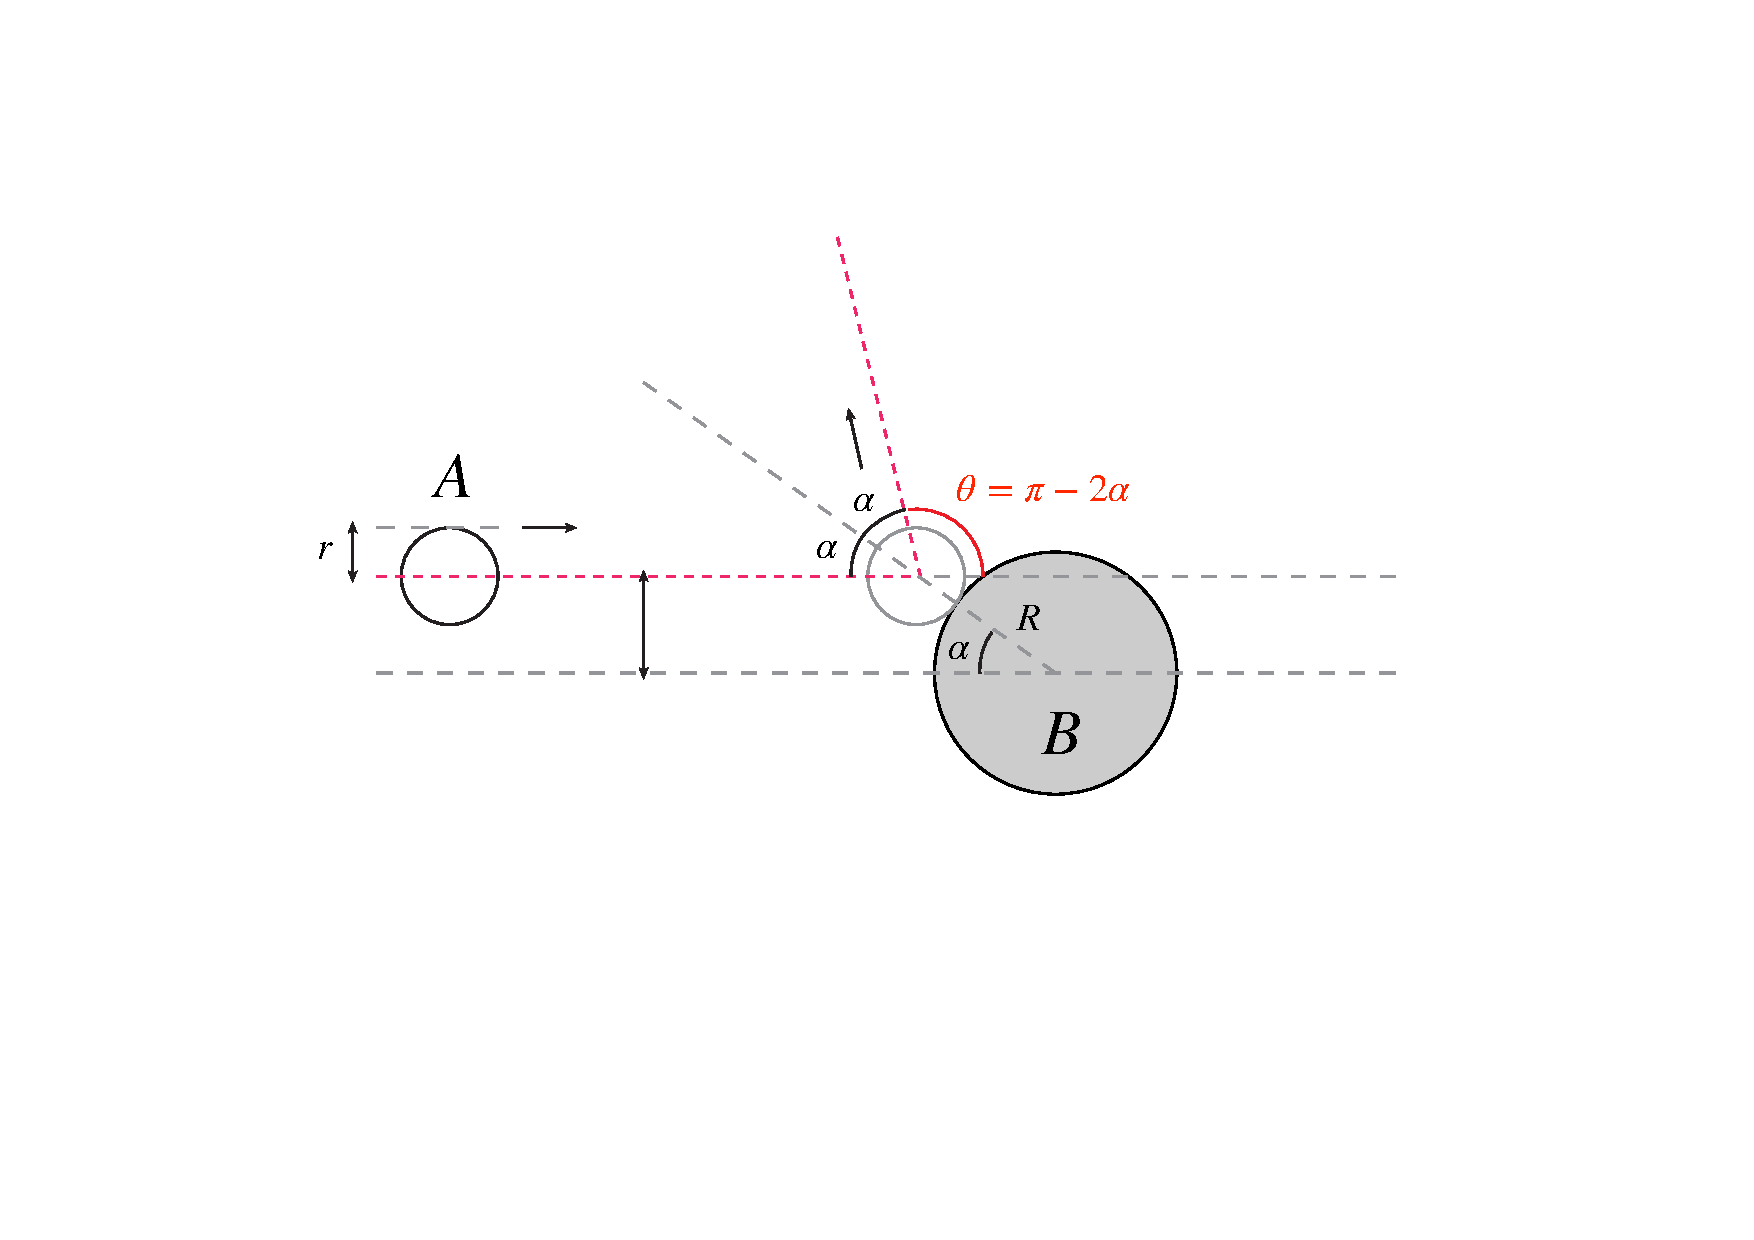
\includegraphics[width=1.0\textwidth]{Scattering-1}
    \caption{(Left) Illustration of the collision of a probe sphere (A) on a target sphere (B), in the rest frame of the target where the probe sphere has an initial velocity {\bf v}. (Right) Illustration of the relation between impact parameter and scattering angle.}
    \label{fig:spheres}
\end{figure}{}

Now, let's suppose that the nature of the target particle $B$ is not known, while that of probes is known to be hard spheres -- similarly to what happens in particle physics experiments. If it were possible to fully control the initial conditions of the incident probe and measure the resulting scattering angle -- for instance by scanning any possible impact parameter and verifying that the corresponding scattering angle $\theta$ follows the law of Eq.~\eqref{eq:spheres} -- this would corroborate the hypothesis that also $B$ is a hard sphere, i.e. the result would be an improved understanding of the nature of the target (which is the goal of the scattering experiment!).

{\it This simple macroscopic situation is unfortunately not what typically happens in a microscopic scattering experiment in atomic, nuclear or sub-nuclear physics}, where a beam of incident probe particles are bombarding an ensemble of targets, as illustrated in Figure~\ref{fig:Scattering-2}. In this case the scattering conditions are not precisely well defined, and the beam and the target are defined by an ensemble of parameters that characterize particles that are approximately in a similar dynamic state. This means that we know that all particles of the beam have similar velocities and masses, and that all targets are considered to be at rest, but we cannot "follow" individually what happens to each of those particles.

The case of \emph{colliding beams} (which is how scattering experiments at the highest energies are conducted, for example at the Large Hadron Collider at CERN) is equivalent to the case of \emph{fixed-target experiments}, as in the rest frame of one beam the collisions can be considered on fixed target. ``Colliders'' and colliding beams will be discussed briefly in Section~\ref{sec:colliders}.

The essential difference with a perfectly known beam of probe particles is that the impact parameter for each specific collision is not known. This impossibility, or in other words the non-perfectly-measurable nature of scattering experiments, has two possible fundamental origins which are completely different in nature:
\begin{itemize}
    \item Classical impossibility: a practical or experimental impossibility to measure the motion of all single particles and their trajectories.
    \item Quantum mechanics: at quantum scales, from the uncertainty principle, it is inherently impossible to  know with arbitrary precision the quantum observables which are canonic conjugates (like momentum and position, or energy and time).  
\end{itemize}

In this context, where the individual collision cannot be measured (i.e. where the individual impact parameter is not known), other observables are required to describe the dynamics of collisions.


\section{Main Definitions and notion of cross section}

Let's consider a case of a beam of particles of type $A$ colliding on a target made of particles of type $B$. We choose the reference frame in which the $B$ particles  are at rest and the $A$ particles  are traveling towards the target with a velocity $\vec{v_A}$. The transverse size of the beam of  $A$ particles is characterized by the surface ${S}$. This picture describes the laboratory frame view of a typical {\it fixed target} experiment. As mentioned in the previous section, the case of {\it colliding beams} -- where a beam of $B$ particles are traveling with a velocity $\vec{v_B}$ towards $A$ -- is fully equivalent, and just requires a change of reference frame to yield the same picture, by transforming any vector $\vec{u}$ as 
\(\vec{u} \rightarrow \vec{u} -\vec{v_B}.\)
Therefore $\vec{v_A}' = \vec{v_A}-\vec{v_B}$ and  $\vec{v_B}' = \vec{0}$. For head-on collisions, i.e. collisions where angle between the two colliding beams is zero, one simply has $v_A' = v_A+v_B$. 

We therefore assume in the following the {\it fixed target} picture, and consider a scattering experiment as illustrated in Fig.~\ref{fig:Scattering-2}, where a cylindrical beam of particles of type $A$ and surface $S$ travels with velocity $\vec{v}_A$ towards a target whose length along the beam direction is $d$, and whose transverse size is sufficient to fully contain the incoming beam.
To characterize the initial conditions of the experiment, let's first define two important quantities for modeling the scattering process.

\begin{figure}
%    \centering
    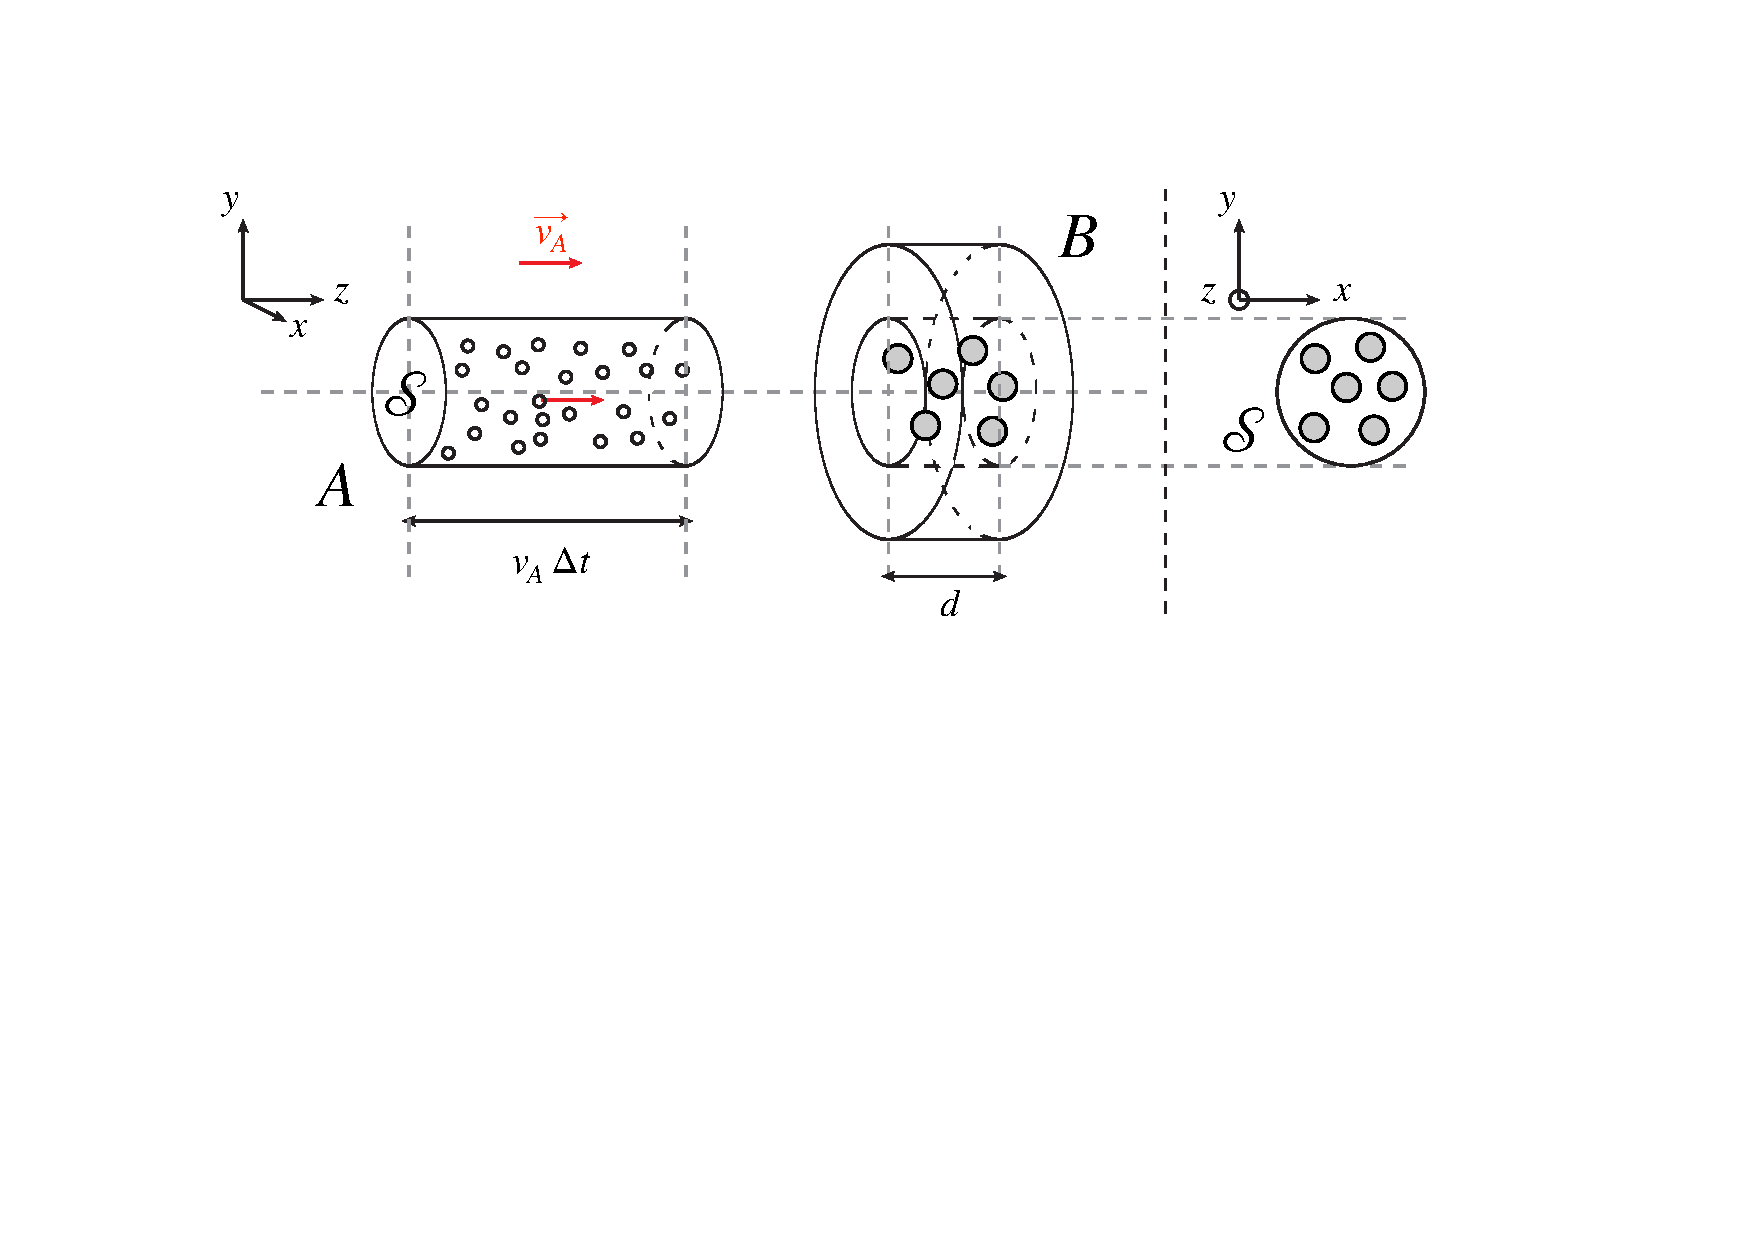
\includegraphics[width=1.0\textwidth]{Scattering-2}
    \caption{Illustration of a scattering process between a beam of surface $S$, made of particles of type $A$ and velocity $\vec{v}_A$, and a target made of particles of type $B$. The length of the target along the beam direction is $d$, and its transverse size is sufficient to fully contain the incoming beam. Left: three-dimensional view; right: view on the plane transverse to the beam direction (usually referred to as ``transverse plane'').}
    \label{fig:Scattering-2}
\end{figure}{}

\definition{{\bf The flux of beam particles $\phi_A$}: The number of particles of a beam $A$ that traverse a plane perpendicular to their motion, per unit surface and unit of time.}

The flux $\phi_A$ can be expressed in formulas as
\begin{equation*}
\begin{split}
\phi_A & =  \frac{\Delta N_A}{\Delta t} \times \frac{1}{S} \\
& =  \frac{\Delta N_A}{\Delta t \times S \times v_A} \times v_A,
\end{split}
\end{equation*}
where $\Delta N_A$ is the number of particles $A$ in the volume $S v_A \Delta t$. If we introduce the density of particles $A$ of the beam, $n_A$, we have

$$ \boxed{\phi_A = n_A \times v_A. }$$

The other important definition, in this {\it fixed target} view, is the number of targets that are ``seen'' by the beam, which can also be expressed in terms of the density of  $B$ particles, $n_B$, as

\[ \boxed{N_B = n_B \times S \times d.}\]

$N_B$ and $\phi_A$ characterise the initial conditions of the scattering experiment. 


Now, in order to gather information about the nature of the interacting particles or about the interaction itself, the result of the scattering experiment is simply expressed as a number of counts per unit time, i.e. a {\bf rate}. This concept will be further developed in the next section; in order to get there, we first need to introduce a concept which is best understood with the simple geometrical example of colliding spheres: the concept of {\bf scattering cross section}.

What we are looking for is the best way to quantitatively describe the interaction between two particles $A$ and $B$ from the main observable of a scattering experiment, the scattering rate $\od{N_I}{t}$.

For the simple example of scattering sphere, let's first estimate the number of interactions of a particle $A$ during a short time interval $\Delta t$. Considering that the particle $A$ is taken at random {\it uniformly} in the beam volume $S \times v_A \times \Delta t$, the number of targets that the particle $A$ will ``see'' during this time will simply be $n_B \times S \times v_A \Delta t$.

\begin{figure}
    \centering
    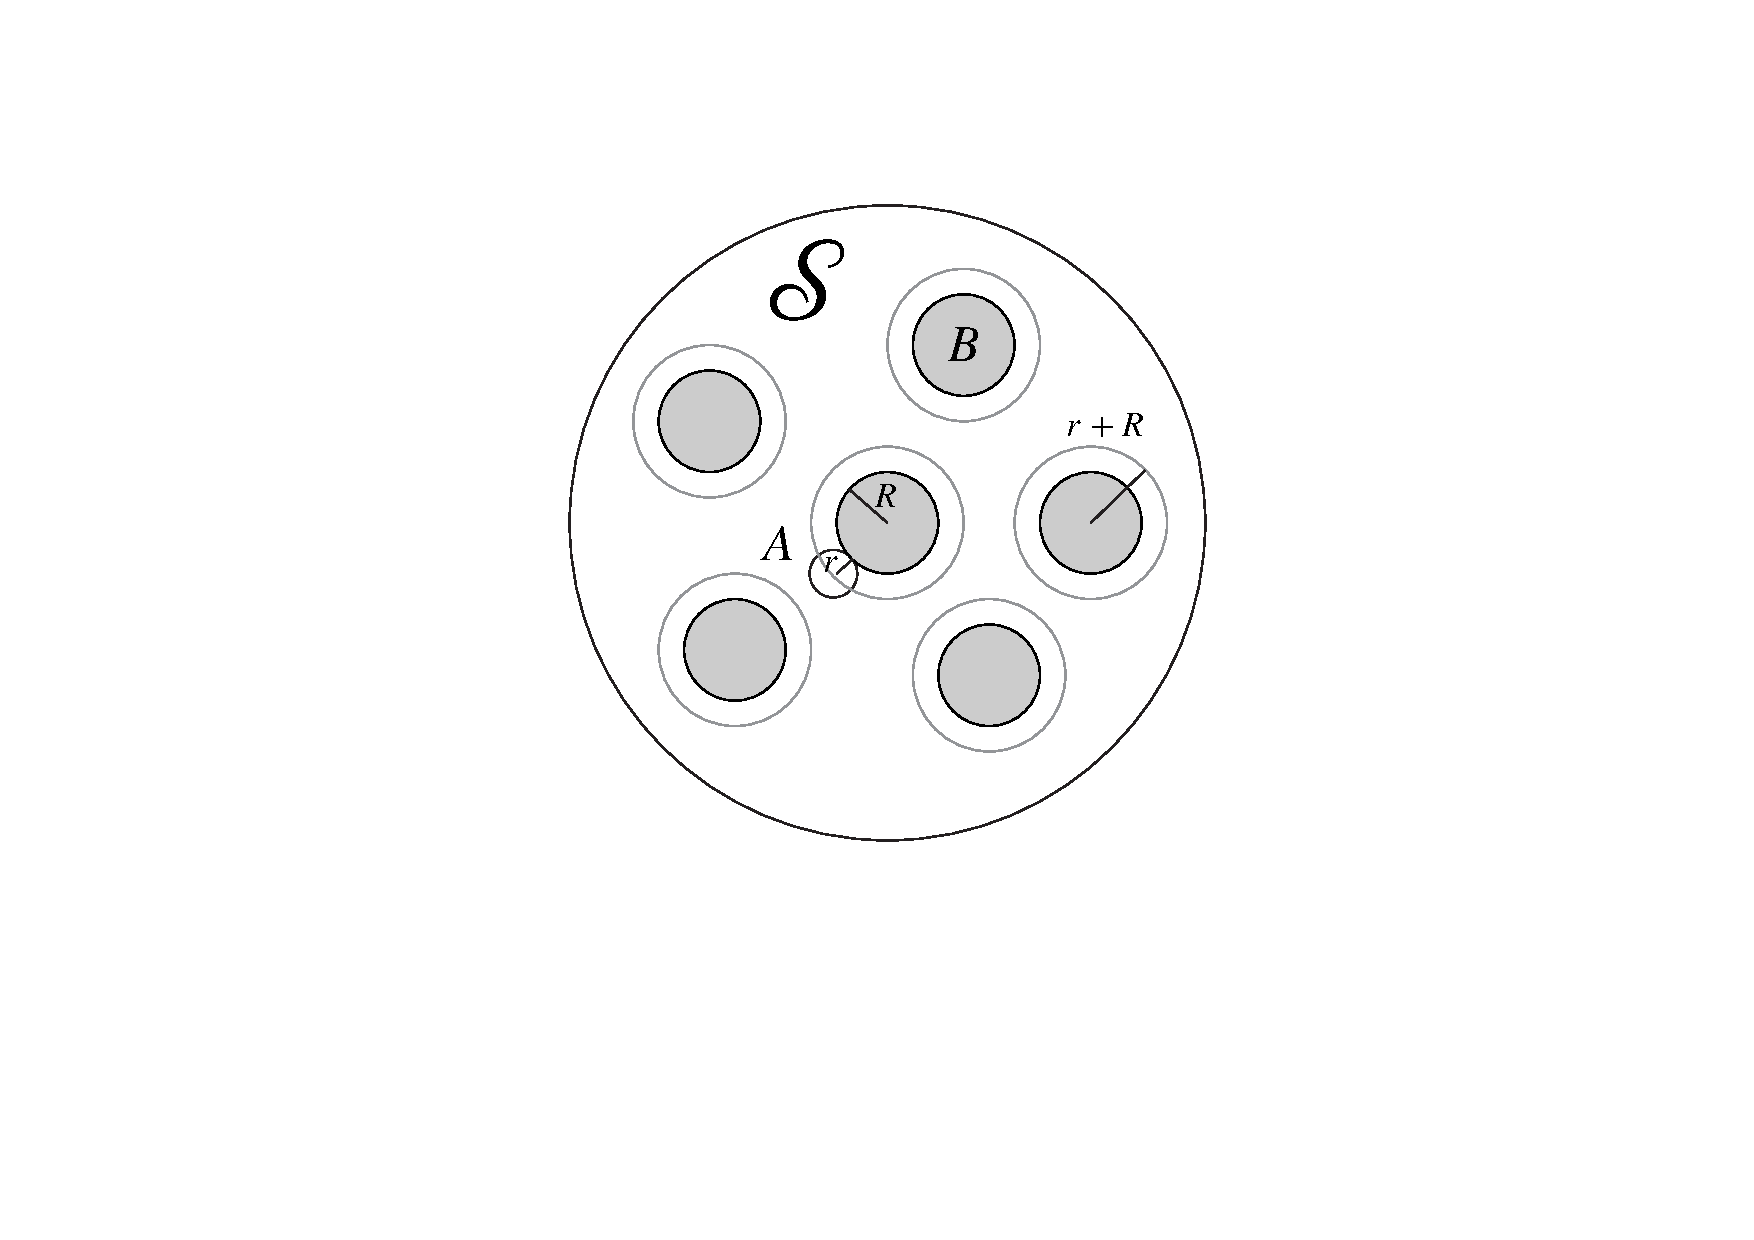
\includegraphics[width=0.4\textwidth]{Scattering-3}
    \caption{Illustration of the available scattering surface within the surface area of the beam. This transverse view corresponds to a slice of width $v_A \Delta t$.}
    \label{fig:Scattering-3}
\end{figure}{}

Let us compute, for each particle $B$, the probability for $A$ and $B$ to interact, by considering the distribution of $A$ and $B$ to be uniform over the slice of the beam, and considering that a contact between the spheres will occur if the impact parameter $b$ will be smaller than $r+R$. The probability $\delta P$ of the two to be in contact will simply be the ratio between the ``contact'' surface and the entire surface of the beam, i.e.

\[ \delta P = \frac{\pi (r+R)^2}{S} \equiv \frac{\sigma}{S}, \]

\noindent where $\sigma = \pi (r+R)^2$. For a given $A$ particl to interact with \emph{any}  $B$ particle within the slice of beam considered, the probability of an interaction $\Delta P$ will then be

\[ \Delta P = \delta P \times n_B v_A S \Delta t.\]

The next step is to extend the calculation to the beam traversing the entire width of the target $d$ -- which requires that the beam length is longer than the target. The total number of $A$ particles that can interact is then $n_A \times S \times d$.

The number of interactions per unit time for a beam crossing the target will thus be

\[\frac{\Delta N_I}{\Delta t} =\frac{\Delta P}{\Delta t} \times N_A= \frac{\Delta P}{\Delta t} \times n_A \times S \times d. \]

The {\bf rate} of interactions will therefore be:

\begin{align*}
\frac{\Delta N_I}{\Delta t} & =  n_A \times S \times d \times n_B \times v_A \times \sigma \\
& =  (n_A v_A) \times (n_B \times S \times d) \times \sigma.
\end{align*}

This simple equation describes how the rate of events can be expressed in terms of the initial conditions of the beam and the target and the cross section which describes the probability of an interaction between a particle $A$ and a particle $B$ as a fraction of the surface area of the beam.


\definition{{\bf The scattering cross section} is defined for any scattering process by generalising the geometrical description of the example above: the cross section is the quantity  $\sigma$ which allows to express the rate of a scattering process as

$$ \boxed{ \frac{\Delta N_I}{\Delta t}  =  \phi_A \times N_B \times \sigma}.$$

}

Cross section has the units of a surface.
In the processes relevant for nuclear and subnuclear physics, cross sections are typically of the order of magnitude of the size of nuclei -- for instance as $^{238}U$, which was deemed to be {\it "as big as a barn"}. This defines the typical unit of cross section, i.e. $10^{-28}$~m$^2$:

$$\boxed{1 \; {\rm barn} = 1 \; {\rm b} = 10^{-28} \; {\rm m^2} }.$$

Another important definition which further simplifies the equation defining the cross section is that of luminosity.

\definition{{\bf Luminosity}: the luminosity $\mathcal{L}$ determines the initial conditions of the scattering experiment, and is defined as
$$\boxed{\mathcal{L} = \phi_A \times N_B }.$$

Luminosity is often expressed in units of $[\mathcal{L}]=\si{cm^{-2}s^{-1}}$.
}

\section{Differential Cross Section}\label{sec:sfererigide}

In order to be able to fully characterise the interaction, it is important to measure all measurable properties of the scattered particles (i.e. reconstruct the final state of the interaction fully). When the nature of the particle is known, the measurable quantities for a scattering experiment are its direction and energy in the final state (assuming that knowing its nature means knowing its mass and therefore its momentum is fixed). Typically the cross section is then measured in a differential fashion, by counting the number of particles per unit time (i.e. the rate) as a function of the particle's energy and direction in spherical coordinates $(E,\theta, \phi)$. 

A typical scattering experiment is illustrated in Fig.~\ref{fig:Scattering-4}, where a detector measuring a small portion of solid angle $d\Omega$ is considered.

\begin{figure}
%    \centering
    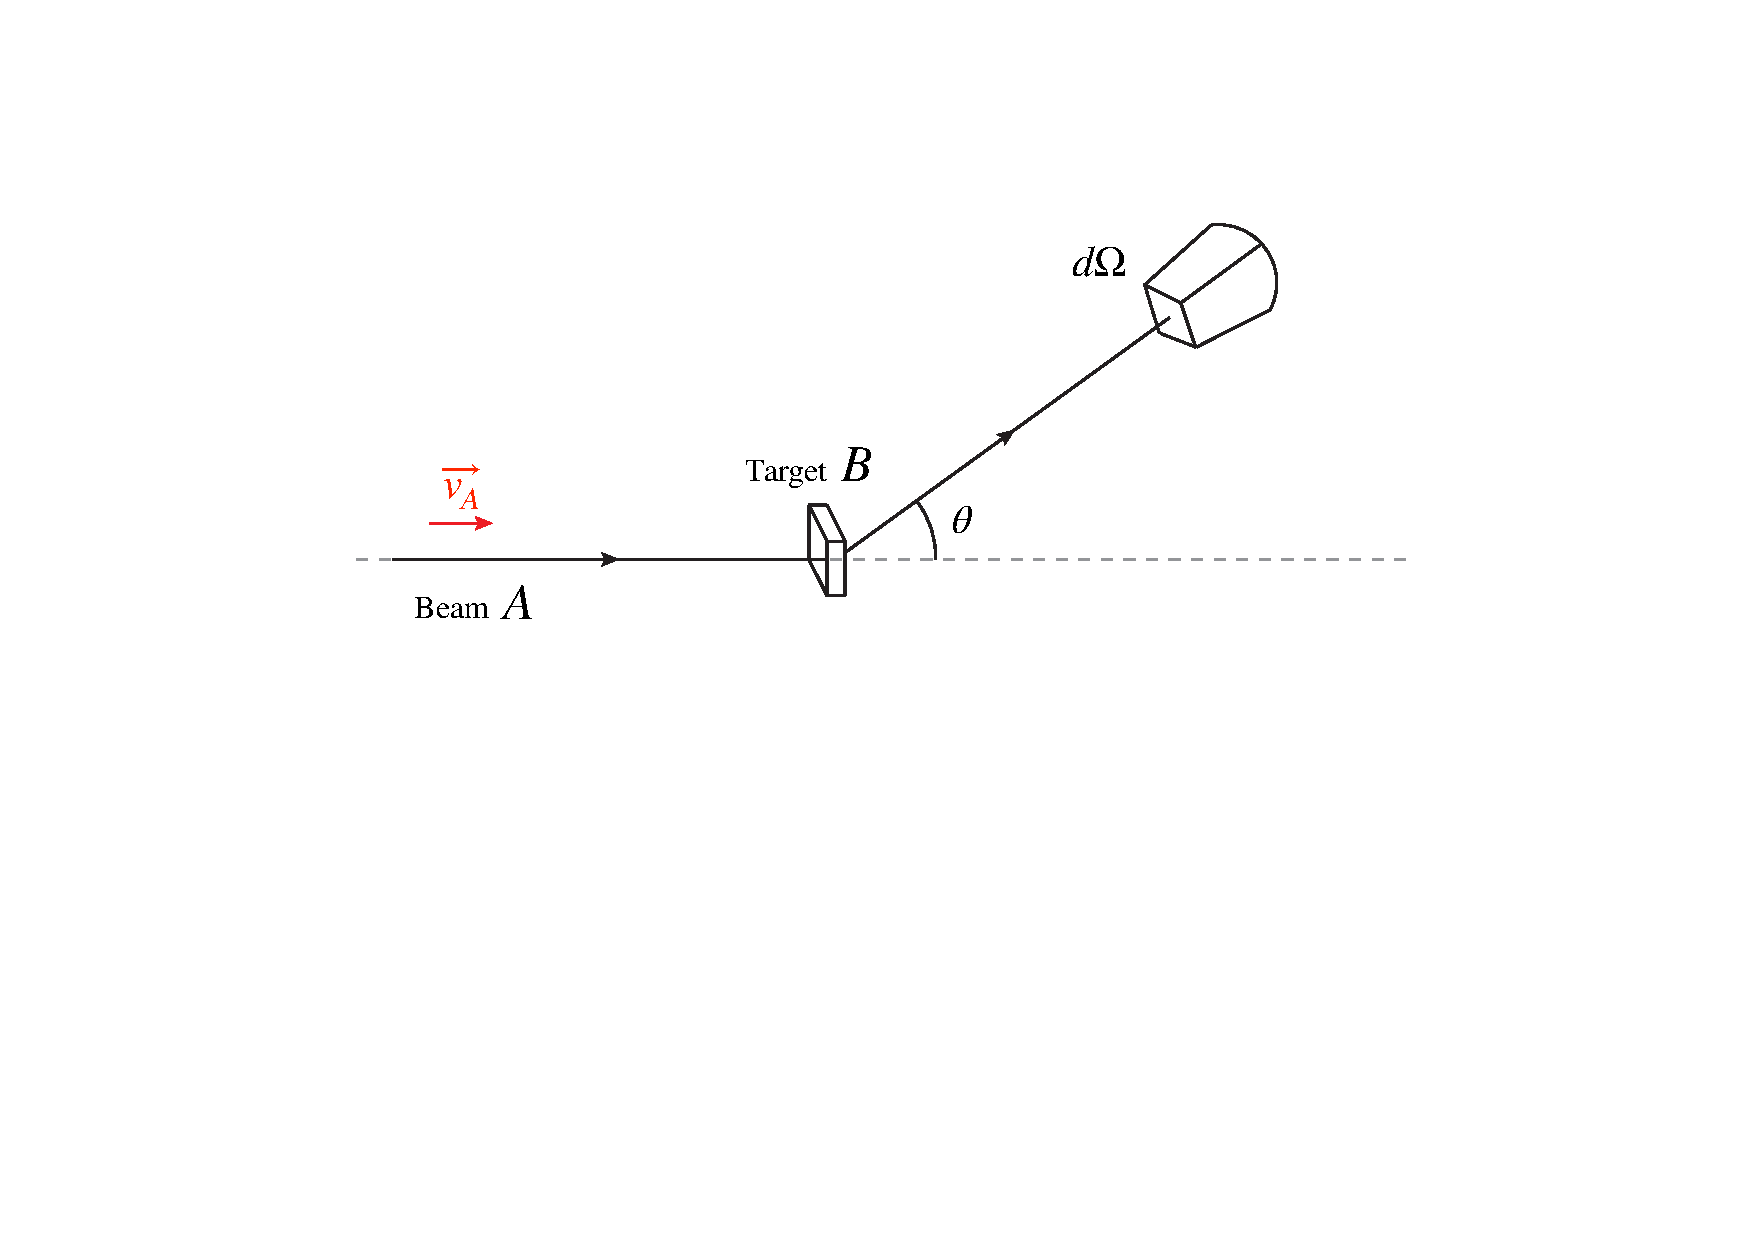
\includegraphics[width=0.9\textwidth]{Scattering-4}
    \caption{Illustration of a typical scattering experiment measuring a differential cross section $\sigma(E, \theta, \phi)$ of the scattering of particles of type $A$ on a target of particles $B$.}
    \label{fig:Scattering-4}
\end{figure}{}

The differential cross section will then be defined again with respect to the rate of specific scatterings in the $(E,\theta, \phi)$ phase space, yielding

\[
\frac{\Delta N_I}{\Delta t} (E,\theta, \phi) = \dot{N}_I (E,\theta, \phi) = \phi_A N_B \sigma (E,\theta, \phi).
\]

Given that the differentiation comes from the phase space in the final state, the only dependence that relates the initial state to the final state being the cross section (as $\mathcal{L}$ is a constant), one can then write
\[\frac{d^3\sigma}{dE d\theta d\phi}(E,\theta,\phi) = \frac{d^3 \dot{N}_I 
(E,\theta,\phi)}{dE d\theta d\phi} \times \frac{1}{\mathcal{L}}.\]
Or, in other typical cases where there is a cylindrical symmetry (uniform scattering in the azimuthal angle $\phi$) and a scattering where the final state energy of the measured particle is fixed, then the relevant quantity will be
\[\frac{d\sigma}{d\Omega}(\theta) = \frac{d \dot{N}_I}{
d\Omega}(\theta) \times \frac{1}{\mathcal{L}}.\]
From this differential cross section, the interaction rate at a certain scattering angle $\theta$ within a solid angle $d\Omega$ can be derived. In all of these cases, we are always doing the same thing: expressing the probability of the interaction in terms of quantities which define the ``parameter space'' in which we measure the scattering (i.e. the interaction rate). Choosing with respect to which variables we express the differential cross section is a matter of knowing how the scattering experiment is conducted -- whether our particle detectors cover the full solid angle or not, whether we measure energies or angles or we can assume some symmetry of the system, etc.

We can then return to the simple case of colliding spheres and compute the prediction of the differential cross section.

As we have seen in this case, the energy or velocity of the scattered sphere is constant and equal in norm to the initial velocity $v_A$. The scattered spheres will be uniformly distributed in the azimuth direction $\phi$ -- there is no reason for them to prefer any specific value of $\phi$. We can then compute the differential cross section as a function of the polar scattering angle $\theta$, which will correspond to a specific element of solid angle $d\Omega$ that can be integrated over $\phi$. We have seen that  a given scattering angle $\theta$ corresponds to a specific value of the {\it impact parameter} $b$. The scattered particles $A$ will be in the element solid angle $d\Omega$ if the impact parameter $b$ lies in the interval $[b, b+db]$. If we look at the collision in the transverse plane with respect to the beam direction (Fig.~\ref{fig:Scattering-5}), this allows to estimate the probability of an interaction in these conditions, which corresponds to the ratio between the area of the ring and the total surface, $2\pi b db/S$. Following the same reasoning as for the total cross section, one can write the contribution to the total rate corresponding to this ``ring'' as
\[
d \dot{N}_I = d \sigma (b) \times \phi_A \times N_B,
\]
where according to Fig.~\ref{fig:Scattering-5} one has
\[d\sigma (b) = 2 \pi b db.\]

\begin{figure}
    \centering
    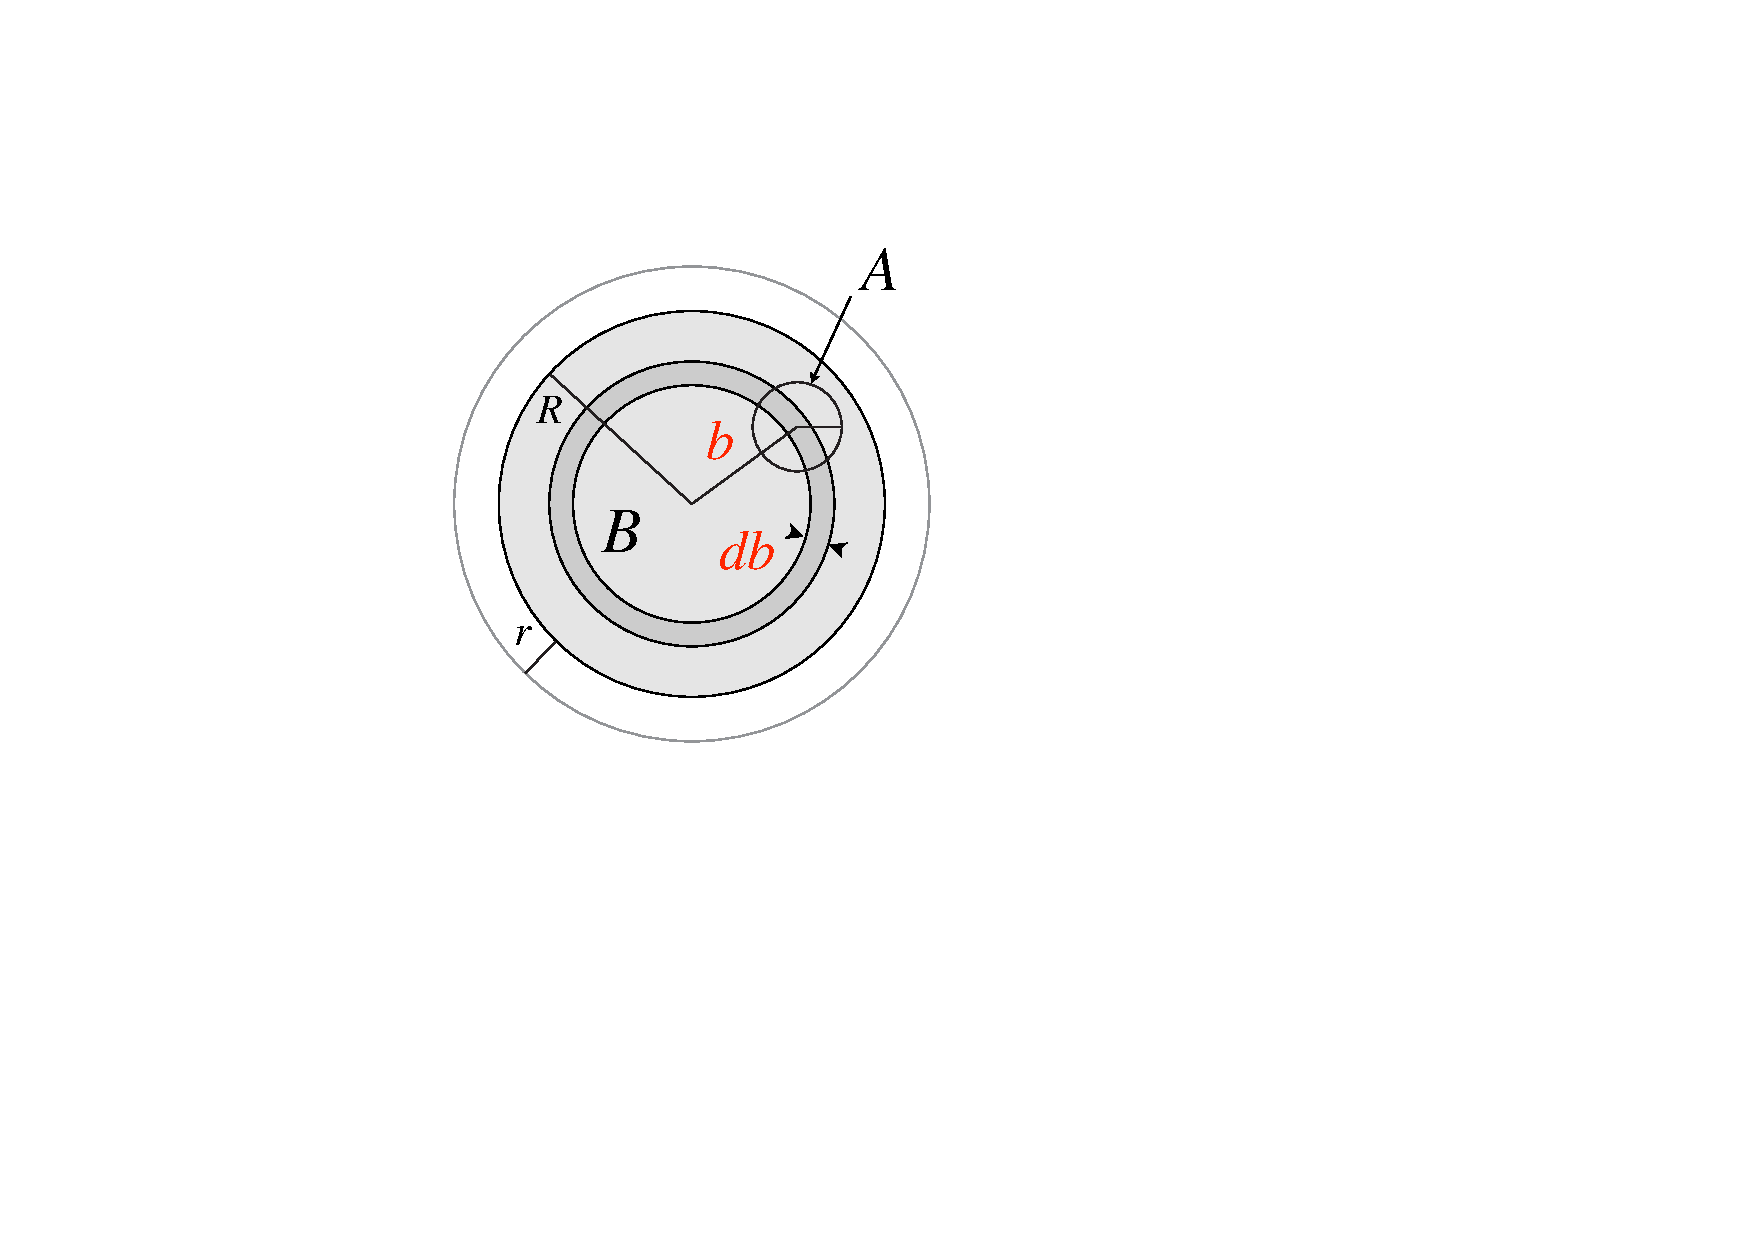
\includegraphics[width=0.5\textwidth]{Scattering-5}
    \caption{Illustration (in the shaded area) of the surface area representing the cross section for a scattering corresponding to an impact parameter $b$ and its corresponding scattering angle.}
    \label{fig:Scattering-5}
\end{figure}{}

Then the differential rate can be written from the relation between the impact parameter and the scattering angle $b=(R+r) \cos \frac{\theta}{2}$:

\begin{align*}
    d \dot{N}_I & = 2 \pi (R+r) \cos \frac{\theta}{2} \times \mathcal{L} \times db \\
    &= 2 \pi (R+r) \cos \frac{\theta}{2} \times \mathcal{L} \times \left | \frac{db}{d\theta} \right  | d\theta \\
    &= 2\pi (R+r)^2 \frac{1}{2} \cos \frac{\theta}{2} \sin \frac{\theta}{2} \times \mathcal{L} \times d\theta \\
    &= 2 \pi \sin \theta \times \frac{(R+r)^2}{4} d\theta \times \mathcal{L}.
\end{align*}
Here used the relation between the impact parameter and scattering angle, from which one has
\[\od{b}{\theta} = \frac{R+r}{2}\od{ \cos \frac{\theta}{2}}{\theta} = - \frac{R+r}{2} \sin \frac{\theta}{2}.\]

Now, let us consider an element solid angle in spherical coordinates $d\Omega = \sin \theta d\theta d\phi$. Since scattering is uniform in the azimuthal angle $\phi$, the element solid angle can be expressed as

\[ d\Omega = \sin \theta d\theta \int_0^{2\pi} d\phi = 2\pi \sin \theta d\theta,\]
and the differential rate can be written as
\[\od{\dot{N}_I}{\Omega} = \frac{(R+r)^2}{4} \times \mathcal{L},\]
so that the differential cross section is
\[\frac{d \sigma}{d \Omega} = \frac{(R+r)^2}{4}.\]
This implies that the distribution of the scattering of two spheres is uniform in any direction! The rate measured by a detector will be the same in any direction. 

We can then see for consistency what happens when the differential cross section is integrated over the entire solid angle:
\[ \sigma = \int_0^{4\pi} \left ( \frac{d\sigma}{d\Omega} \right ) d\Omega = \pi (r+R)^2,\]
which is precisely the initial result for the total cross section $\sigma$.

The reasoning we followed here in the simple, ideal example of colliding hard spheres is the same which is used in any scattering experiment. The task will be to determine which quantities are measured in the final state, and to calculate the differential and total cross-section of the interaction -- which is in general a measurement of its probability, rather than of the ``physical size'' of the involved particles.

\section{Absorption Coefficient and Mean Free Path}

In this section the important notions of absorption coefficient and mean free path will be introduced. These two concepts will prove essential for describing quantitatively what happens when particles travel through matter. %These notions will be very important in Chapter~\ref{}. 

\subsection{Absorption coefficient}
Let us consider a beam of particles $A$ on a target of particles $B$. The probability for a given particle of a beam to interact on a element distance $dx$ will be constant,
\[dP = \sigma n_B dx,\]
where $n_B$ is the density of particles $B$. We can then define the quantity
\[\mu = \sigma n_B,\]
so that the variation in the flux of the beam on a length $dx$ can be written as
\[d\phi = -\phi dP = -\phi \mu dx,\]
therefore
\[ \frac{d\phi}{\phi} = -\mu dx \; \; {\rm i.e.} \; \; [log \phi]_{\phi_0}^{\phi} = -\mu x,\]
or 
\[\boxed{\phi(x) = \phi_0 e^{-\mu x}.}\]
The dimensions of $\mu$ will then be those of the inverse of a length, as $[\mu]=[\sigma][n_B] = \si{m^2} \times \si{m^{-3}} = \si{m^{-1}}$. 

\definition {\textbf{The absorption coefficient} is defined as the product between the cross section and the number of targets per unit volume,

\[ \mu = \sigma n_B.\]

The \textbf{attenuation length} $\lambda$ is defined as its reciprocal, i.e.

\[ \lambda = \frac{1}{\mu}.\]}

The attenuation length corresponds to the length after which the flux of incoming particles gets reduced by a factor $e$ (i.e. where $\phi(x=\lambda) = \phi_0 / e$).

\subsection{Mean free path}
The mean free path is the average distance covered by a particle in a target between two successive interactions. Let us then first consider a distance $x$ along the path of the particle from a point $O$ with coordinate $0$ in the $x$ direction. The distance $x$ represents the distance between two interactions (or ``scatterings''), one occurring at $0$ and the subsequent occurring at $x$.

In order to compute the probability of having a distance $x$ between two scatterings, one has to follow two steps. 
First the probability for the probe particle {\it not to have interacted} between $0$ and $x$ ($P_{NI}(x)$) can be computed from integrating its differential form
\[ dP_{NI}(x) = P_{NI}(x+dx) - P_{NI}(x), \; \; {\rm where} \; \; P_{NI}(x+dx) = P_{NI}(x) (1 -\mu dx),\]
which means that the probability of not having interacted in $x+dx$ can simply be deducted from the probability of not having interacted in $x$. Then, one has
\[dP_{NI}(x) = -\mu \, dx \, P_{NI}(x) \; \; \Longrightarrow \; \; \left[\ln P_{NI}\right]_{0}^{x} = \mu \, x.\]

Assuming that $P_{NI}(0) = 1$, the probability of {\it not having interacted} in $x$ will then be
\[P_{NI}(x) = e^{-\mu \, x}.\]
The probability of interacting after $x$ (but not before!) will then be
\[P(x)\, dx = P_{NI}(x) \times \mu \, dx = \mu e^{-\mu \, x}\, dx.\]
If we average all the possible path lengths $x$ weighted by their probability, we get the average path:
\begin{align*}
    \langle x\rangle & = \int_0^{\infty} x \cdot P(x) dx \\
    & = \int_0^{\infty} x  \mu e^{-\mu \, x}dx \\
     & = \frac{1}{\mu} \int_0^{\infty}  (\mu \, x) e^{-\mu \, x} d(\mu \,x) \\
     &= [-e^y (1+y)]_0^{\infty} \; \; \qquad (y=\mu \, x) \\
     &= \frac{1}{\mu},
\end{align*}
where the integration is simply done by parts.

\definition{{\bf The mean free path} of a particle is the average length traveled by a particle between two subsequent interactions,
\[\langle x\rangle = \lambda.\]
}
One can immediately see that the mean free path is equivalent to the attenuation length, as defined in the previous section.

\section{The Rutherford Scattering Experiment} 

These definitions can be immediately applied to the analysis of one of the most fundamental, landmark experiments for our understanding of atoms: the Rutherford experiment. 

\subsection{Early atomic model} 

Towards the turn of the XX century, it was understood that the atom was made of positive charges and electrons. Thomson then proposed the idea of a dynamic model where the electrons -- which were understood to be particles after his own experiment -- would be embedded in a volume filled with a positively charges. Thomson considered three hypotheses on how the electrons could be distributed with respect to the positive charges. The first was that the electrons were embedded in a uniformly positively-charged medium, the second was to pair each electron with a positive charge and the third was that the negatively-charged particles would orbit inside a volume of positive charges. Thomson retained the first hypothesis as the most likely. This model is often referred to as the ``plum pudding'' model, where the electrons are modelled as ``plums'' evenly distributed within a ``pudding'' or positively-charged continuum (see an illustration of the ``plum pudding"model'' on the left of Fig.~\ref{fig:RutherfordAtom}).

\begin{figure}
    \centering
    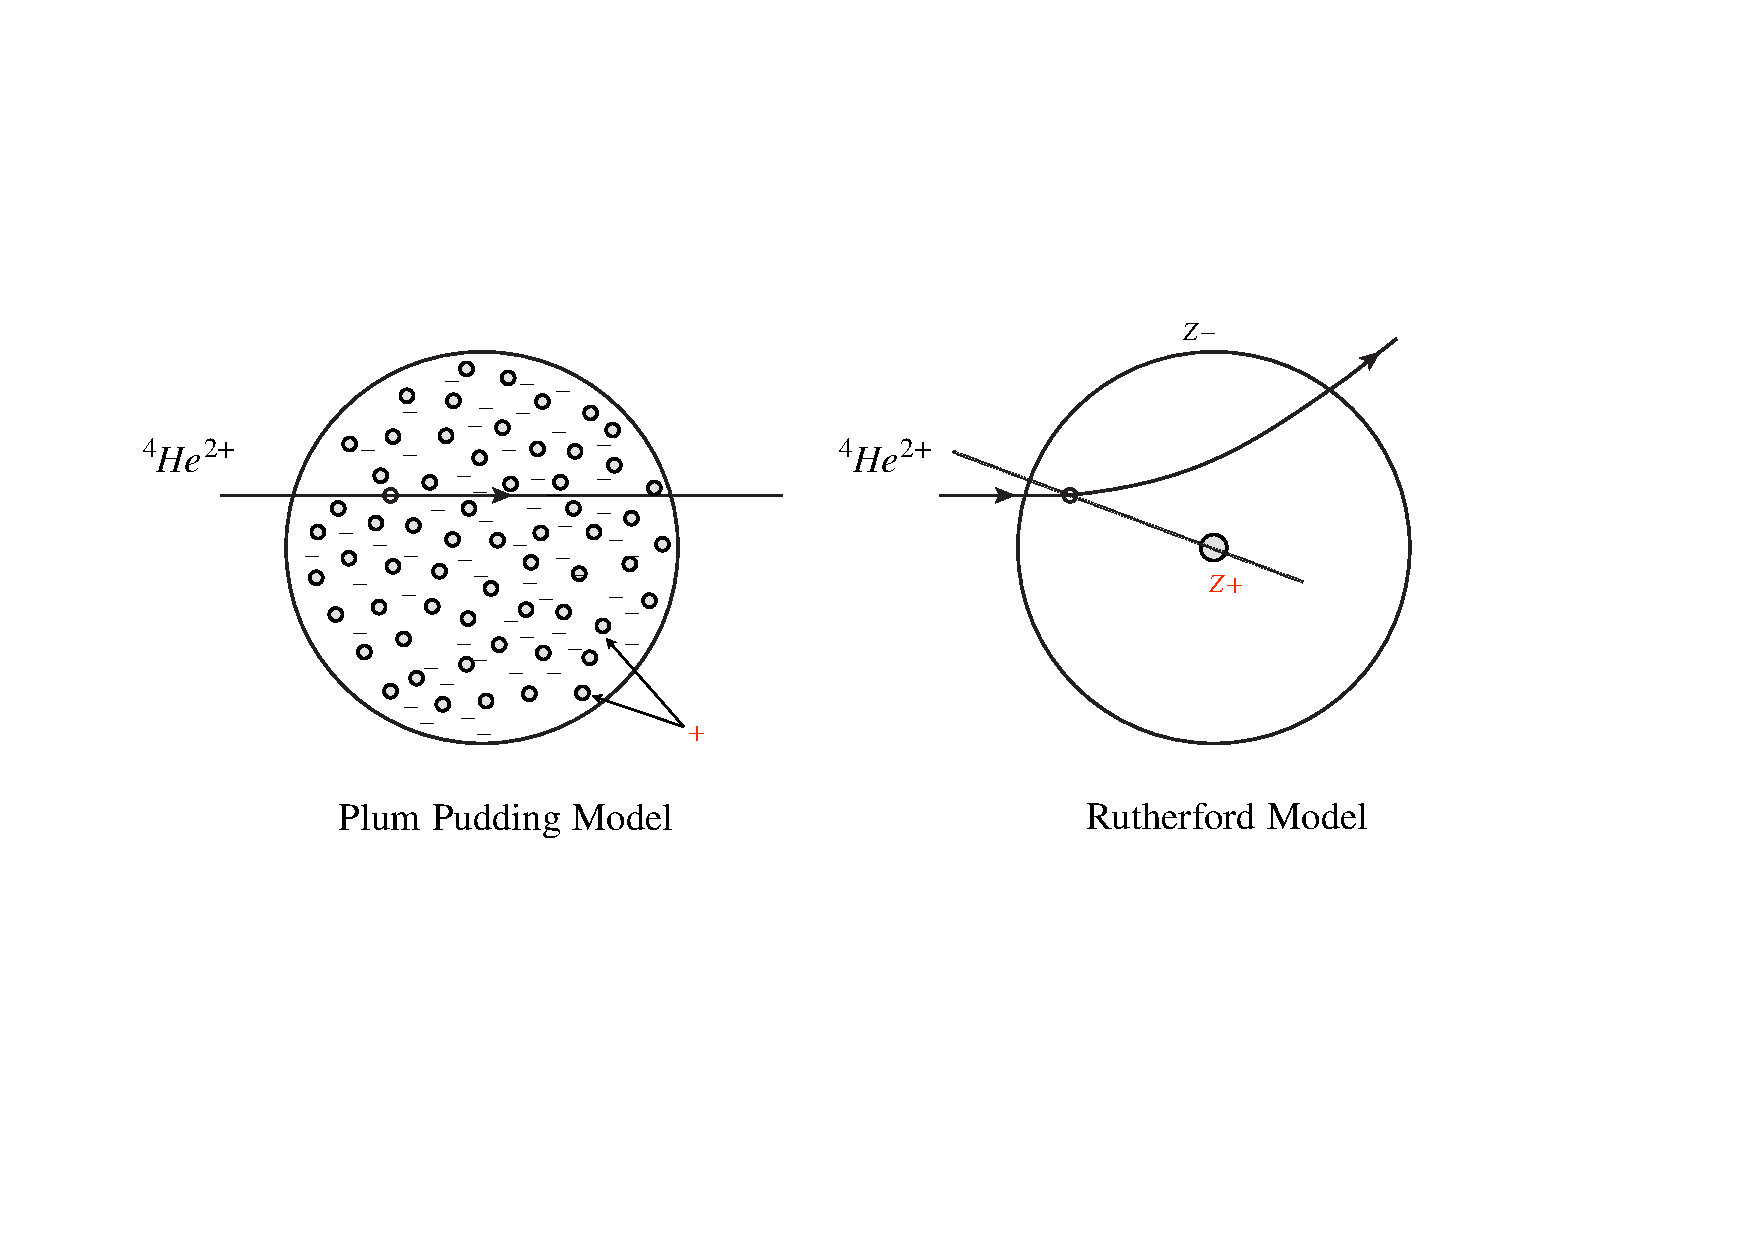
\includegraphics[width=0.9\textwidth]{Scattering-7}
    \caption{(Left) Early atomic model by Thomson and illustration of an $\alpha$ particle traversing it unperturbed. (Right) Illustration of the Rutherford model where all positive charges are concentrated in a positively-charged nucleus at the centre of the atom. The trajectory of an $\alpha$ particle is shown as well.}
    \label{fig:RutherfordAtom}
\end{figure}{}

Thomson encouraged his student at the time, Ernest Rutherford, to pursue experiments to probe models of the atom. In order to do so, they exploited the idea of using $\alpha$ particles ($^4He^{2+}$) to probe the structure of the atom, as shown in Fig.~\ref{fig:RutherfordAtom}. 

In the case of the ``plum pudding'' model (left figure), no deviation of the $\alpha$ particles is expected. This can be understood from the fact that, at any time, the electric field created by the charges in the atom can be separated into two contributions: the first is the outer spherical and hollow shell volume at a radius with respect to the centre of the atom which is larger than the distance of the $\alpha$ particle to the atom's centre, as illustrated in Fig.~\ref{fig:gauss}-a; the second is the inner sphere as illustrated in Fig.~\ref{fig:gauss}-b.

Since the atom is neutral, when the $\alpha$ particle travels outside of the atom it will ``sense'' no electric field. When inside the atom, the contribution of the electric field on the $\alpha$ particle from the outer hollow spherical shell volume is $0$ from Gauss' theorem, as there are no charges inside the inner volume. The component from the inner sphere can be computed as well using Gauss' theorem: one has
\[ \varoiint \vec{E} \cdot d\vec{S} = 4\pi r^2 E \frac{1}{\varepsilon_0} \iiint \rho dV = \frac{Q}{\varepsilon_0} = 0,\]
i.e. the electric field generated by the inner sphere will  also be equal to $0$. In this model the $\alpha$ particle should travel through the atom mostly unperturbed!

In the case where the positive charges are concentrated in a limited volume at the centre of the atom, the situation is quite different. When inside the inner shell of electrons, the $\alpha$ particle will be fully subject to the electric field of the charges at the centre of the atom (see Fig.~\ref{fig:gauss}-b).

\begin{figure}
    \centering
    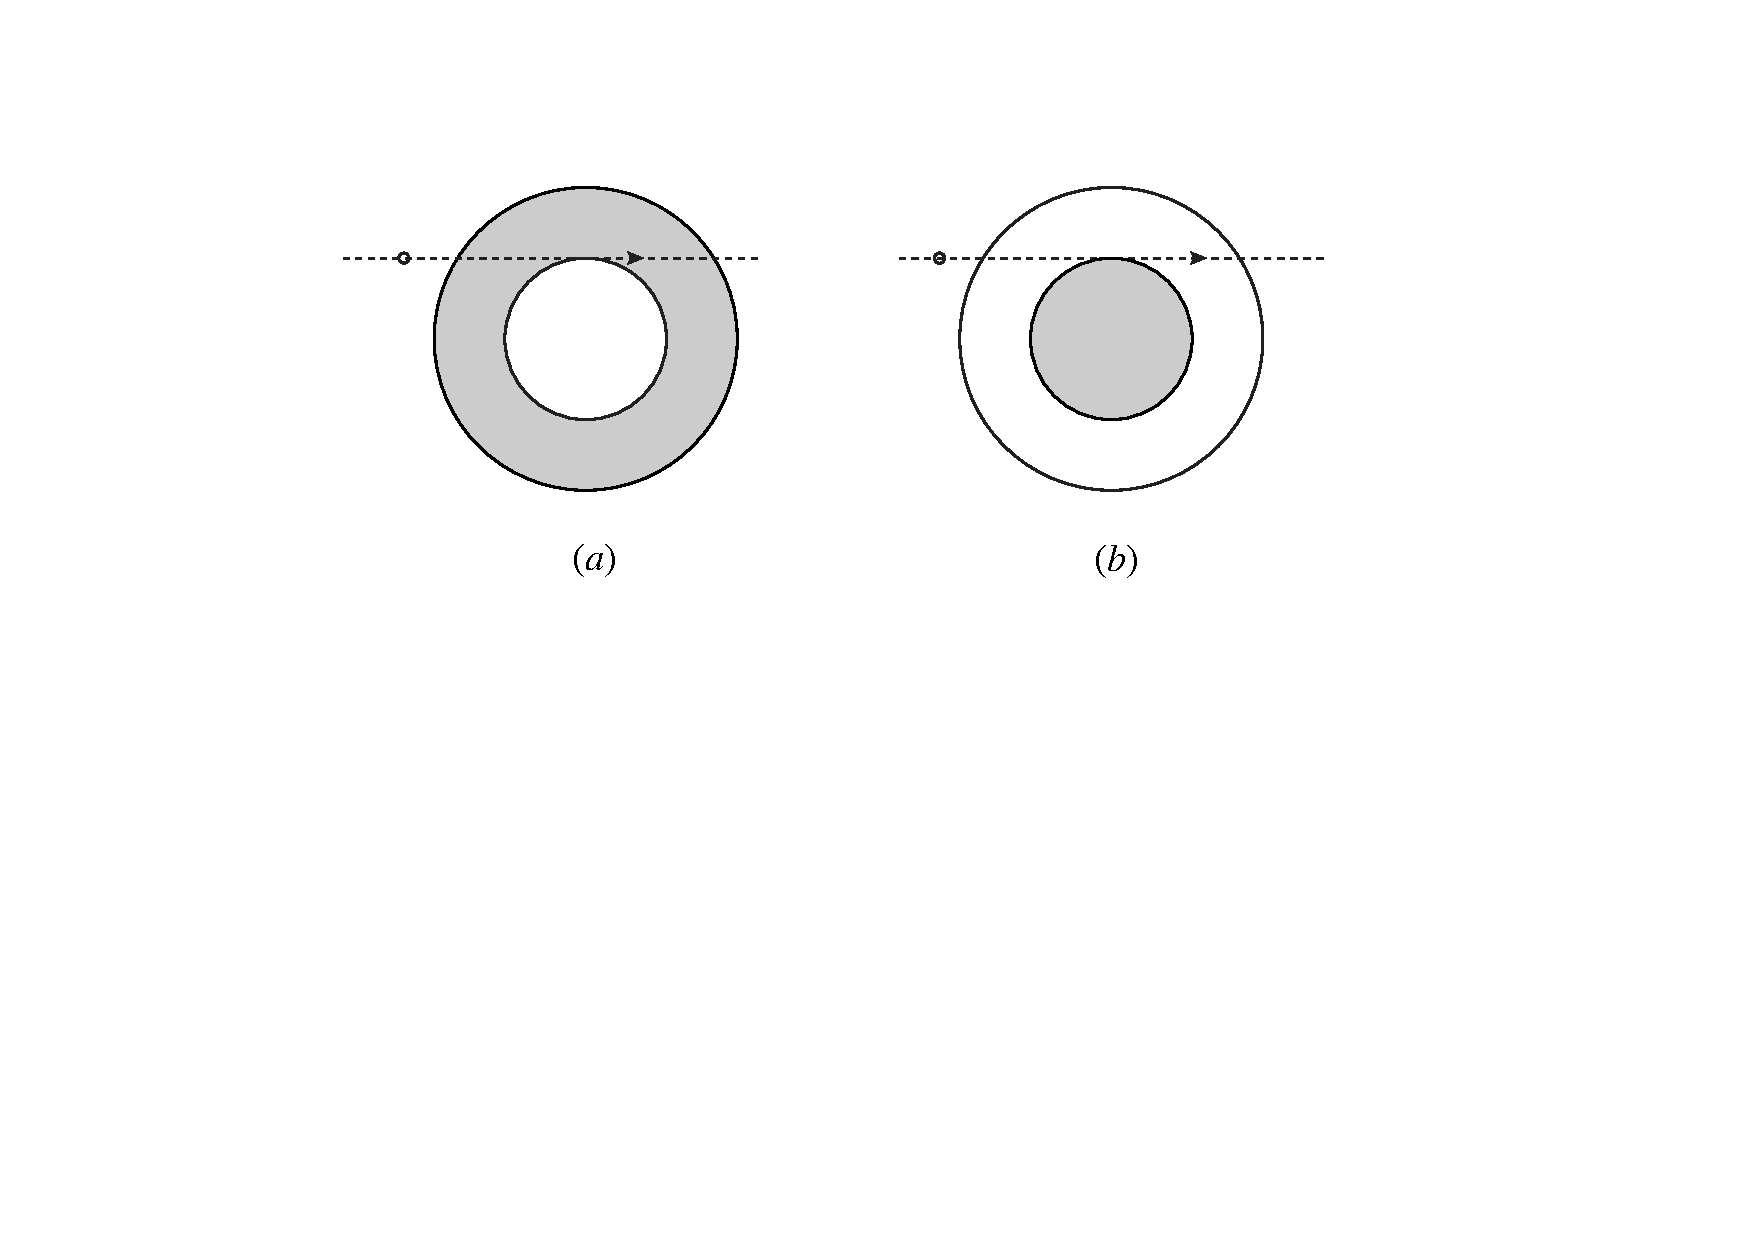
\includegraphics[width=0.9\textwidth]{Scattering-8}
    \caption{Illustration of the two volumes of charges that are considered in order to derive the trajectory of an $\alpha$ particle within an atom in the ``plum pudding'' model.}
    \label{fig:gauss}
\end{figure}{}

\subsection{The Rutherford scattering experiment}

Rutherford started his experiments with Hans Geiger in 1907, joined by Ernest Marsden in 1909 at the University of Manchester. In 1912, the team was joined by Niels Bohr to study the atom.

The setup of the Rutherford-Geiger-Marsden experiment is illustrated in Fig.~\ref{fig:geiger-marsden}. The team used a radium source to generate the beam of $\alpha$ particles, which impinged on a target made of gold foil. The system was designed to measure the scattering at large angles: for this reason, the main detection device (the microscope and the screen) could rotate around the target. The idea of the detector is that the passage of $\alpha$ particles through the screen of zinc sulfate would generate a faint scintillation light that could be visible if the eye was sufficiently accustomed to the dark (which took about half an hour during the experiment). The source generated a "beam" of collimated $\alpha$ particles. 

\begin{figure}
    \centering
    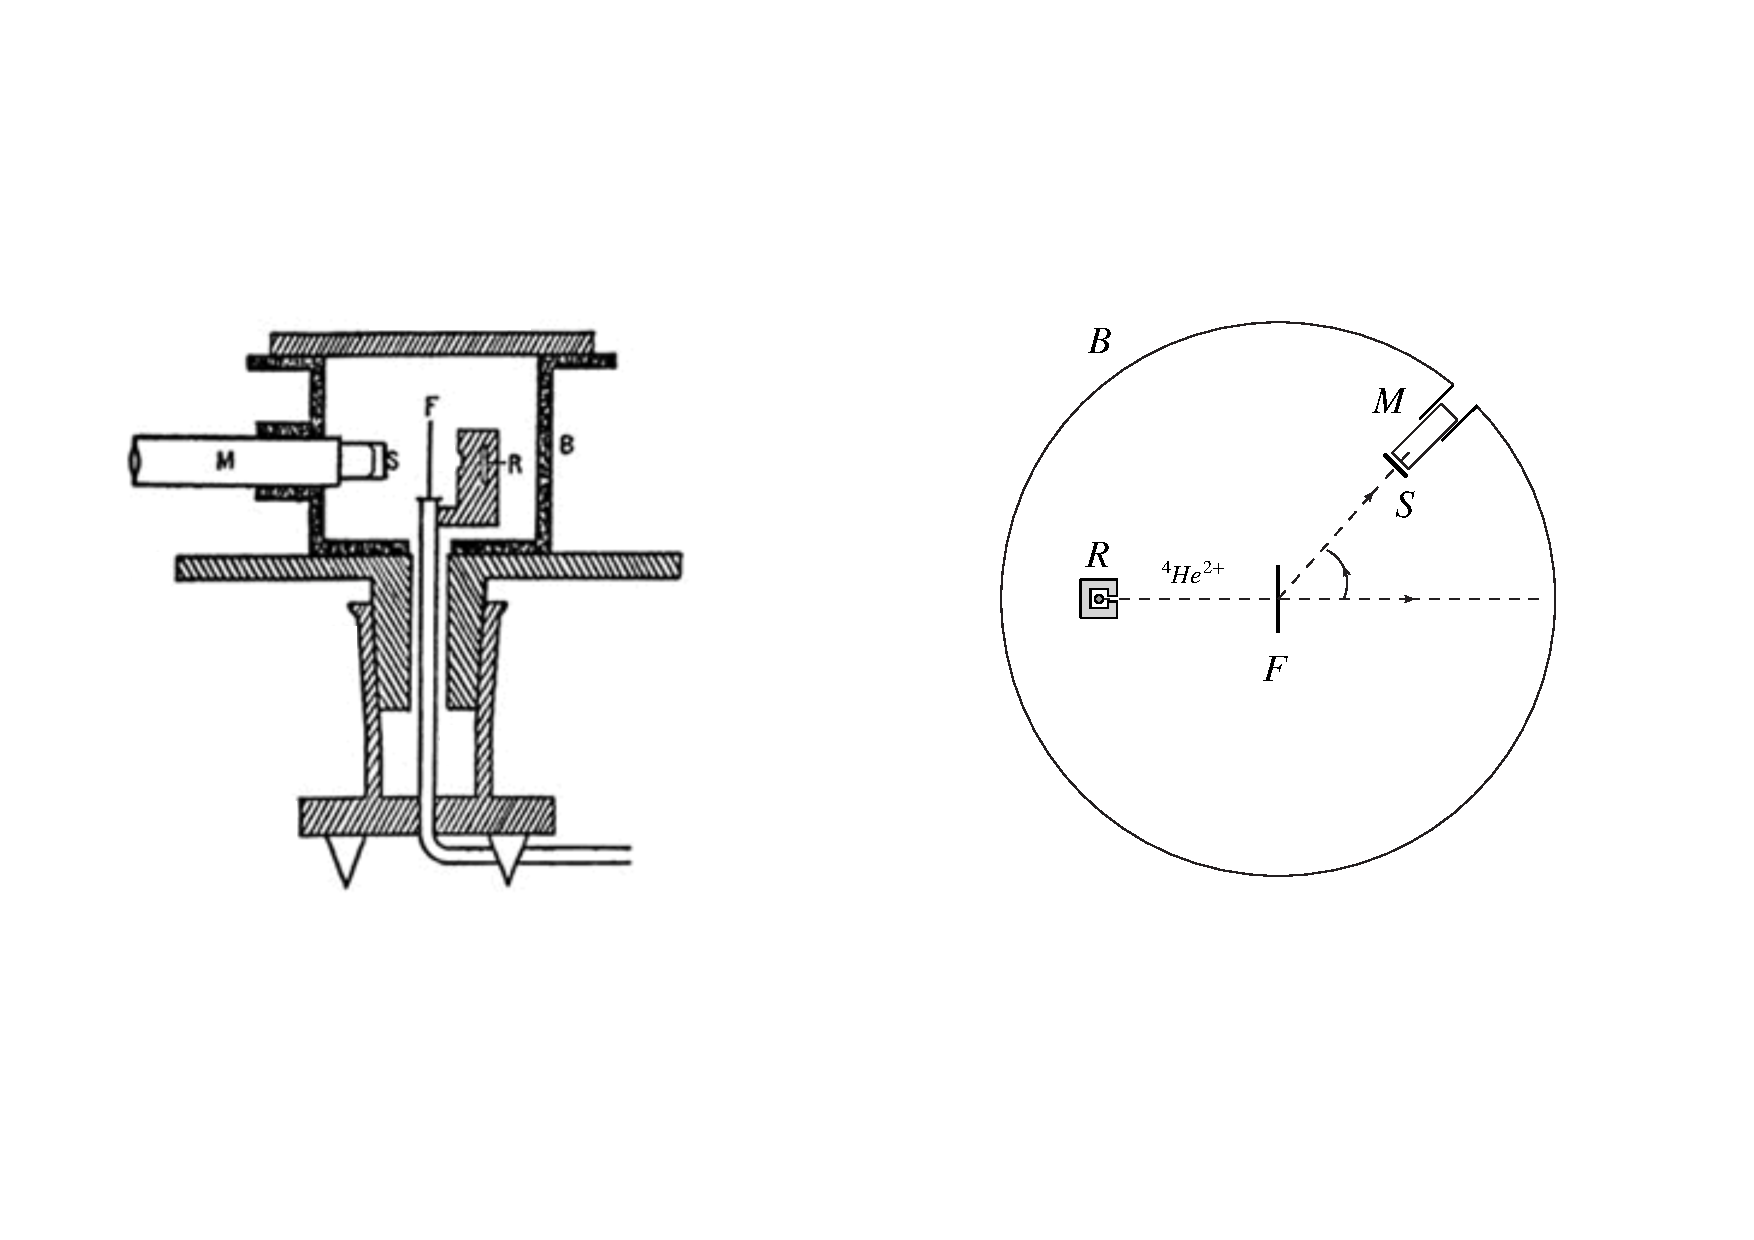
\includegraphics[width=0.9\textwidth]{Scattering-9}
    \caption{(Left) Illustration of the Rutherford-Geiger-Marsden $\alpha$ particles scattering experiment (lateral view). Source: Cambridge University. (Right) A schematic illustration of the principle of the experiment (top view) where the main points are reported:  (R) is the Radium source of $\alpha$ particles, (F) is the target foil, (M) is the microscope for the observation which could rotate along with the cylindrical box (B), (S) was a Zinc Sulfate screen which produced the scintillation at the passage of $\alpha$ particles to be observed by the microscope, and (D) a diaphragm through which the particles were emitted. }
    \label{fig:geiger-marsden}
\end{figure}{}

The result of the experiment was striking, as emphasized by Rutherford's famous quote: ``[The results were] as if you fired a 15-inch shell at a piece of tissue paper and it came back and hit you''. Back-scatterings of $\alpha$ particles were in fact observed.

\subsection{Prediction of the Rutherford Scattering Cross Section}
In order to explain the astonishing results of his scattering experiment, Rutherford proposed a different model for the atom where all the positive charges are concentrated in a small volume at the centre of the atom, and the negative particles (electrons) orbit around this central volume.

Assuming a relatively small volume for this ``nucleus'', when the $\alpha$ particle enters the volume of the atom, again -- according to Gauss' theorem -- the electric field created by the shell of electrons will cancel. The $\alpha$ particle will not ``feel'' the effect of the electrons, while the field from the ``nucleus'' (where the positive charges are concentrated) will act on the $\alpha$ particle as a point source, again according to Gauss' theorem (see the illustration of Rutherford's model in Fig.~\ref{fig:RutherfordAtom}).   
With this model greatly simplified by Gauss' theorem, the scattering cross section can be computed assuming that:
\begin{itemize}
    \item the scattering is elastic;
    \item the target is point-like, with a mass $M$ large with respect to the mass of the probe $\alpha$ particles, and with a charge $Ze$;
    \item the probe particle is $^4 He^{2+}$.
\end{itemize}
The scattering can be described schematically as in Fig.~\ref{fig:RutherfordScattering}, which represents the trajectory of a charged particle in a central potential. By construction it is known that these trajectories can be either open or closed, depending on the initial conditions of the system.

\begin{figure}
    \centering
    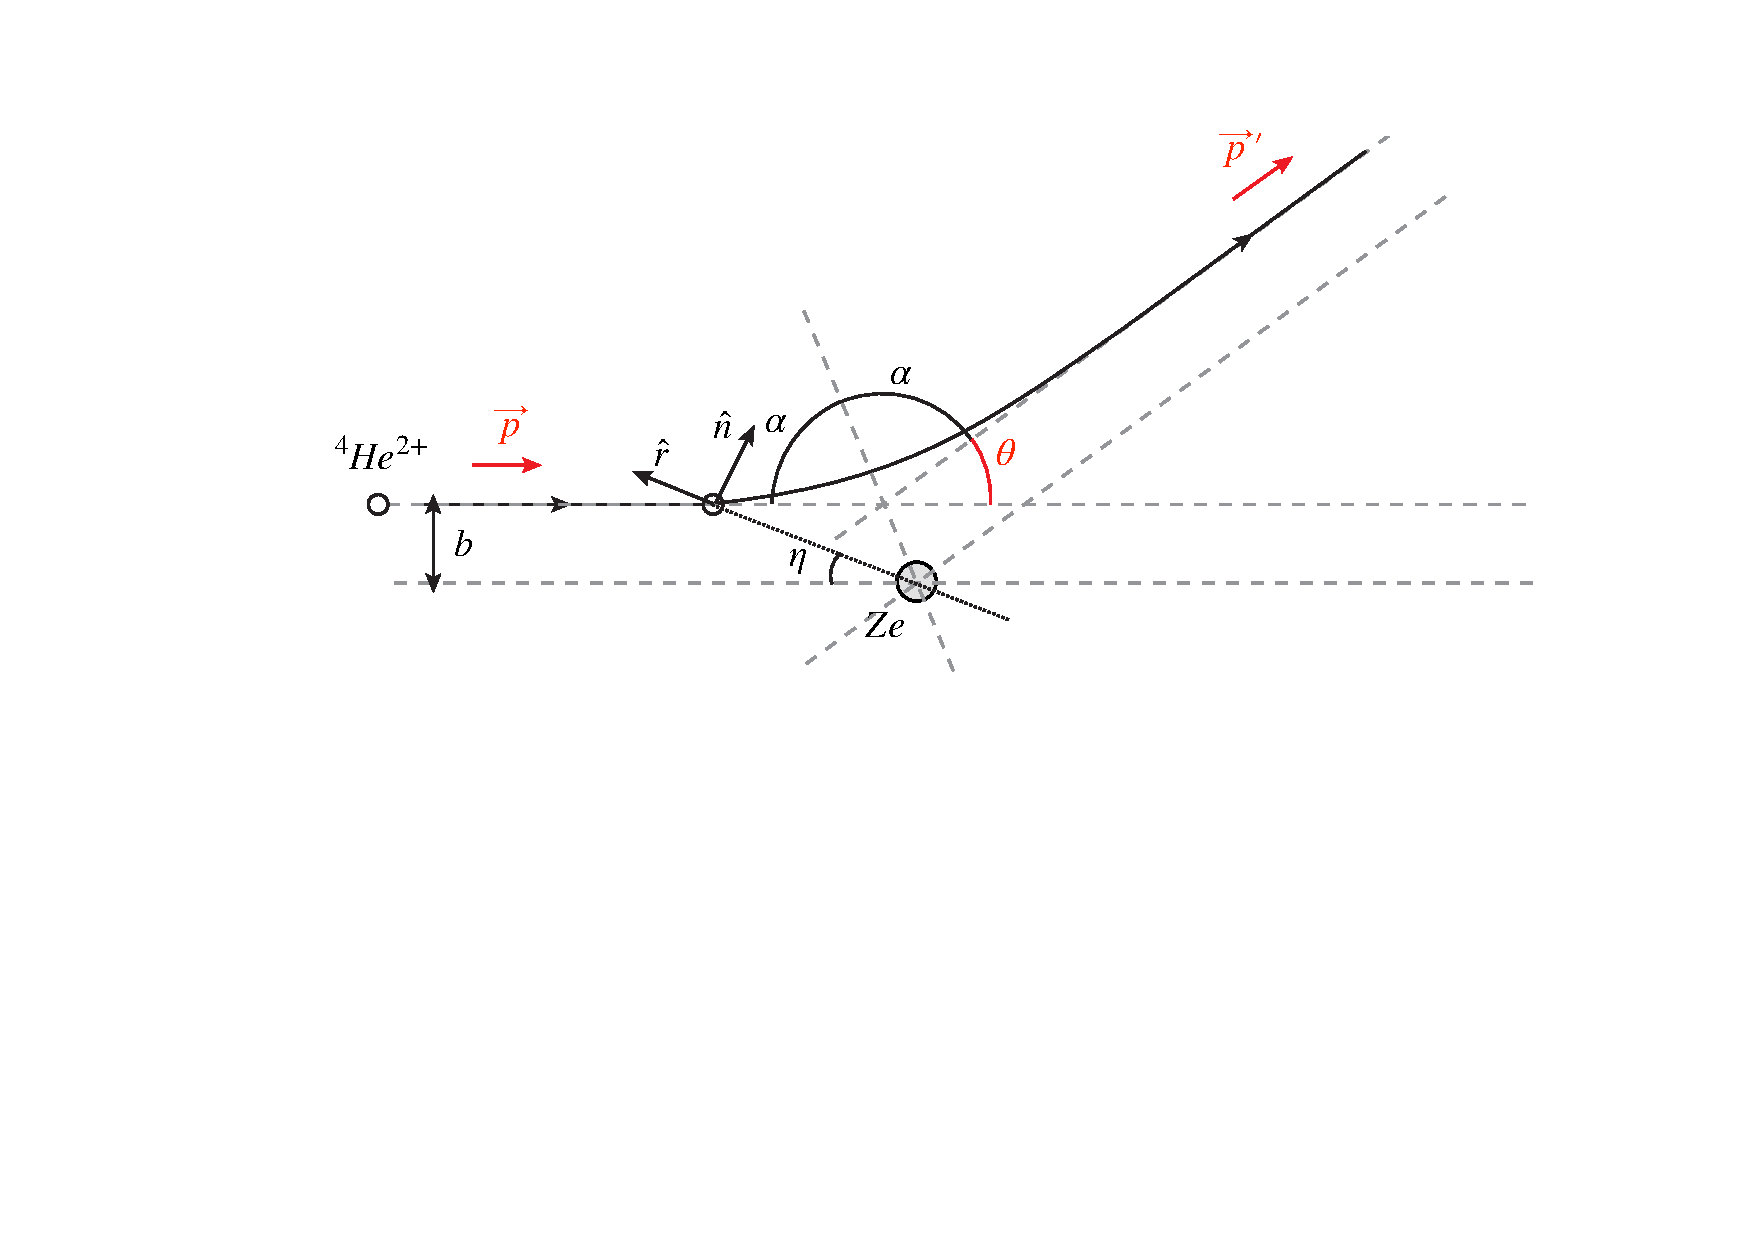
\includegraphics[width=1.0\textwidth]{Scattering-6}
    \caption{Illustration which shows the open hyperbolic trajectory of the $\alpha$ particles deviated from the Coulomb potential of the nucleus.
    In the image, $\theta$ denotes the scattering angle, $b$ the impact parameter of the incoming particle, $p$ is its momentum before the scattering, $p'$ is its momentum after the scattering and $Ze$ is the charge of the nucleus.}
    \label{fig:RutherfordScattering}
\end{figure}{}

In order to compute the cross section of this process, we need to stress an important conceptual point: we are facing a classical, non-relativistic problem which is fully deterministic. This implies that once the relation between the scattering angle and the impact parameter is known, the cross section will be known. The reasoning is precisely the same as that for the collision between hard spheres, where knowing the uniform distribution of the impact parameter probe particles, and using the relation between the impact parameter and the scattering angle, the differential cross section was known. 
The aim of the game will then be to \emph{find the relation between the impact parameter and the scattering angle}. In this case, the calculation will be a tad less straightforward than in the case of the hard spheres.

The first hypothesis is that we are dealing with a central potential,  i.e. that $V(r)$ has only a dependence in $r$. We will also assume that the potential is falling and becomes negligible (or at least its variations are negligible) at long distances. The Coulomb potential is in fact a good example of potential with such properties.
For the Coulomb potential, we know in advance that the trajectory will be a conic with a trajectory that can be open or closed, depending on the initial conditions of the system. As it will become clear in the following, we will be in the framework of an open hyperbolic trajectory. 

Let us define a coordinate system as described in Fig.~\ref{fig:RutherfordScattering}, which is centered in the scattering centre (i.e. the nucleus), which has been assumed to be point-like and is the origin of the potential. Let $\hat{r}$ be the radial unit vector along the direction of the probe particle (an $\alpha$ particle) to the target particle (nucleus); $\hat{n}$ is the normal unit vector. 

Given that the force generated by the potential on the probe particle is radial, its torque will be equal to $0$:
\[
\od{\vec{l}}{t} = \od{(\vec{r}\wedge\vec{p})}{t} = \od{r}{t}\hat{r}\wedge m\vec{v} + \vec{r}\wedge\od{\vec{p}}{t} = \vec{v}\wedge m\vec{v} + \vec{r}\wedge\vec{F} = 0.
\]
Therefore the angular momentum of the probe particle will be a constant of motion,
\[ \vec{\ell} = \vec{r} \wedge m \vec{v} \; \; {\rm thus} \; \; \ell = mrv \sin \eta, \]
where $\eta$ is the angle formed by the vectors $\vec{r}$ and $\vec{v}$. One can then calculate $\ell$ when the $\alpha$ particle is far away from the nucleus, i.e. when $V(r)\rightarrow 0$ and $r\sin\eta=b$, so that
\[
\ell = m r v \sin \eta = m b v_0,
\]
where $v_0$ is the velocity of the particle before scattering. Since energy is conserved, one has immediately

%The angle $\psi$ will relate to the angle $\eta$ through the following relation (see Fig.~\ref{fig:RutherfordScattering}:

%$$ \eta = \pi - \chi - \gamma$$

%Looking at the limit $\eta \rightarrow \pi$, assuming that the angle $\gamma$ will fall rapidly to 0 (which is the case since the electric field outside the atom will be expected to be exactly 0), then

%$$\lim\limits_{\eta \rightarrow \pi} \; |r \sin \eta| \sim r \sin \chi \sim b $$

%Therefore in terms of angular momentum:

%$$\lim\limits_{\eta \rightarrow \pi} \; \ell = \ell_0 = m v_0 b$$

%Where the initial velocity can be expressed in terms of the initial energy of the $\alpha$ particles $E$:

\begin{equation}
\label{eq:E}
E = \frac{1}{2} m v_0^2 \; \; \Rightarrow \; \; v_0 = \sqrt{\frac{2E}{m}}  \; \; \Rightarrow \; \; b^2 = \frac{\ell^2}{m^2v_0^2} = \frac{\ell^2}{2mE},
\end{equation}
i.e. we expressed the impact parameter in terms of conserved quantities, the angular momentum of the particle and its total energy, which are constants of motion.

Since the potential is central, it is convenient to represent the position of the incoming particle, $\vec{r}$, in polar coordinates. One has that $\vec{r}=(x,y)$, with
\[
\begin{cases}
x = r \cos \chi,\\
y = r \sin \chi,
\end{cases}
\]
where $\chi$ is the angle between the horizontal axis and $\vec{r}$. In other words, one has
\[
\vec{r}= r\cos\chi \hat{x}+r\sin\chi\hat{y} = r\hat{r},
\]
where $\hat{r}$ is the unit vector along the direction of $\vec{r}$. The unit vector orthogonal to $\hat{r}$ is
\[
\hat{n} = -\sin\chi \hat{x} + \cos\chi \hat{y},
\]
as it can be seen immediately by checking that $\hat{n}\cdot \hat{r}=0$. One can also note that
\[
\od{\hat{r}}{\chi} = \hat{n}.
\]
As a result, we can express the angular momentum of the particle as
\begin{equation*}
\begin{split}
\vec{l}&=m\vec{r}\wedge\vec{v} = m\vec{r}\wedge\od{\vec{r}}{t} = m\vec{r}\wedge\od{(r\hat{r})}{t}\\& = m\vec{r}\wedge\left[\od{r}{t}\hat{r}+r\od{\hat{r}}{t}\right] = 0+m\vec{r} \wedge \left[r\od{\hat{r}}{\chi}\od{\chi}{t}\right] = mr^2\hat{n}\od{\chi}{t},
\end{split}
\end{equation*}
i.e.
%We can then write for any position of the probe $\alpha$ particle on its trajectory that (in polar coordinates within the scattering plane):

%$$\ell = m |\vec{r} \wedge (\frac{dr}{dt} \hat{r} + r \frac{d\chi}{dt}\hat{n})| = mr^2 \frac{d\chi}{dt}$$

%Therefore we will have the following expression:

\begin{equation}
\label{eq:dchi}
\frac{d\chi}{dt} = \frac{\ell}{mr^2}.
\end{equation}

The source used by Rutherford was radium. The typical $\alpha$ radiation energy is of the order of 5~MeV. The total energy of the $\alpha$ particle will be
\[ E = T + m_{\alpha}c^2 = 4005 \; {\rm MeV} \; \Rightarrow \; \gamma = \frac{E}{m_{\alpha}} \sim 1.\]
The momentum of the $\alpha$ particle will then be
\[ p = \sqrt{E^2 - m_{\alpha}^2c^4} \sim 200 \; {\rm MeV/c} \; \Rightarrow \; \beta \gamma \sim \beta \sim 0.05.\]
The probe particle in the fixed-target reference frame is therefore in a  non-relativistic regime. 

The non-relativistic total energy, taking into account the central potential $V(r)$, can be written as
\[E = \frac{1}{2} m v^2 + V(r) = \frac{1}{2} m \left ( \frac{dr}{dt} \right )^2 + \frac{1}{2} m  r^2 \left ( \frac{d\chi}{dt} \right )^2 + V(r).\]
It is worth stressing the fact that $E$ is a constant of motion, while $V$ is a function of $r$.
From the previous expressions we obtain that
\[\frac{1}{2} m \left ( \frac{dr}{dt} \right )^2 = E - V(r) -\frac{\ell^2}{2mr^2} \; \; \Rightarrow \; \;\frac{dr}{dt} = - \sqrt{\frac{2}{m} \left ( E-V(r)-\frac{\ell^2}{2mr^2} \right )},\]
where we took the negative solution since $r$ decreases in the first phase of the trajectory. Using the expression of the angular momentum as a function of the impact parameter from Eq.~\eqref{eq:E}, we get
\begin{equation}
\label{eq:dr}
\frac{dr}{dt} = - \frac{\ell}{mrb} \sqrt{r^2 \left (1-\frac{V(r)}{E} \right ) - b^2}
\end{equation}

Given the expression of Eq.\ref{eq:dchi}, we can derive the variation of $d\chi$:
\begin{equation*}
\begin{split}
d\chi &= \frac{\ell}{mr^2}dt = \frac{\ell}{mr^2}\od{t}{r} dr \\&= \frac{\ell}{mr^2} \dfrac{dr}{-\dfrac{\ell}{mrb}  \sqrt{r^2 \left(1-\dfrac{V(r)}{E} \right) - b^2}} = \frac{-b dr}{r\sqrt{r^2\left(1-\frac{V(r)}{E}\right)-b^2}}.
\end{split}
\end{equation*}

In order to obtain an expression of the scattering angle $\theta$ as a function of the impact parameter of the particle, we consider the point of closest approach of the particle to the nucleus. In that point of space, denoted as $r=r_0$, the particle will have zero velocity, i.e.

\[
\left.\frac{dr}{dt}\right|_{r=r_0} = 0.
\]

This condition is satisfied if the argument of the square root of Eq. \eqref{eq:dr} vanishes, from which we get a relation between the impact parameter and the distance of closest approach,
\[r_0^2 \left ( 1 -\frac{V(r_0)}{E} \right ) - b^2 = 0.\]
This allows us to write
\[ \int_0^{\alpha} d\chi = \alpha = \int_{\infty}^{r_0} \frac{-b dr}{r \sqrt{r^2 \left (1-\dfrac{V(r)}{E} \right ) - b^2}},\]
where we used the fact that the particle comes from infinite distance ($\alpha=0$) and reaches $\alpha$ for $r=r_0$.

From the relation $2\alpha+\theta = \pi$ (which is evident from the symmetry\footnote{This is simply a consequence of the conservation of momentum of the incoming particle.} of  Fig.~\ref{fig:RutherfordScattering}), we get
\[\alpha = \frac{\pi}{2} - \frac{\theta}{2},\]
from which we obtain:
\begin{equation}
\label{eq:generalintegral}
\theta = \pi - 2b \int_{r_0}^{\infty} \frac{dr}{r \sqrt{r^2 \left (1-\dfrac{V(r)}{E} \right ) - b^2}}.
\end{equation}
This formula is valid for every scattering subject to a central potential $V(r)$.

Now let's use the fact the interaction between the $\alpha$ particle and the nucleus is given by the Coulomb potential. The $\alpha$ particle ($^4 He^{2+}$) has charge $z=2$, and we have
\[ V(r) = \frac{zZe^2}{4 \pi \varepsilon_0 r}.\]

In order to simplify the notation, let us define the constant $A = \dfrac{zZe^2}{4 \pi \varepsilon_0 E}$. Then the general central potential integral of Eq.~\eqref{eq:generalintegral} becomes
\begin{equation}
    \label{eq:coulombintegral}
    \theta = \pi - 2b \int_{r_0}^{\infty} \frac{dr}{r \sqrt{r^2 \left (1-\dfrac{A}{r} \right ) - b^2}}.
\end{equation}
We express the distance of closest approach for the Coulomb potential as
\begin{align}
    \left(1-\frac{A}{r}\right)r^2 = b^2\\
    r^2-Ar-b^2=0\\
    r=\frac{A\pm\sqrt{a^2+4b^2}}{2}=\frac{A}{2}\left(1 + \sqrt{1 + \frac{4b^2}{A^2}}\right)\equiv r_0,\label{eq:rutherfordclosestapproach}
\end{align}
where we took the physical solution of the second-order equation (positive sign before the square root).

To solve the integral of Eq.~\eqref{eq:coulombintegral}, we perform the change of variable $x=\frac{1}{r}$, i.e. $dx=-\frac{dr}{r^2}$. We obtain
\[ \theta = \pi - 2b \int_{r_0}^\infty \frac{-dx r^2}{r\sqrt{\frac{1}{x^2}\left(1-Ax\right)-b^2}} = \pi + 2b \int_{x_0}^{0} \frac{dx}{\sqrt{ 1 - A x - b^2 x^2}},\]
where we called $x_0=1/r_0$.

This integral can be computed from the general inverse trigonometric integral
\[ \int \frac{dx}{\sqrt{a +bx +cx^2}} = \frac{1}{\sqrt{-c}} \arccos \left ( -\frac{b+2cx}{\sqrt{b^2-4  ac}} \right ),\]
so that
\begin{equation}
    \label{eq:intacos}
     \theta = \pi + 2b \cdot \frac{1}{b} \left [ \arccos \left ( \frac{A+2b^2x}{\sqrt{A^2 + 4b^2}} \right ) \right ]_{x_0}^{0}
\end{equation}

The lower integration boundary $x_0$ can be written as
\[ x_0 =\frac{1}{r_0} = \frac{2}{A}\frac{1}{\left ( 1 + \sqrt{1 + \frac{4b^2}{A^2}} \right )}.\]
If we define $y = \frac{4b^2}{A^2}$, the argument of the $\arccos$ simplifies greatly:

$$ \frac{A+2b^2x_0}{\sqrt{A^2+4b^2}}=\frac{1+ \dfrac{y}{\left (1 + \sqrt{1+y} \right )}}{\sqrt{1+y}} = \frac{1 + \sqrt{1+y} + y}{\sqrt{1+y} + 1 + y} = 1.$$

Eq.~\eqref{eq:intacos} can then be written in a simple form, by evaluating the upper bound of the integral:
\[ \theta = \pi + 2 \left[ - 2\arccos(1)\right] + \arccos \left (\frac{1}{\sqrt{1+y}} \right ).\]
Taking the cosine and squaring the above expression yields
\[\cos ^2 \left ( \frac{\theta-\pi}{2}\right ) = \frac{1}{1+\dfrac{4b^2}{A^2}}= \sin ^2 \frac{\theta}{2},\]
from which we obtain
\[ \frac{4b^2}{A^2} = \frac{1-\sin ^2\frac{\theta}{2}}{\sin ^2 \frac{\theta}{2}} = \frac{\cos ^2\frac{\theta}{2}}{\sin ^2 \frac{\theta}{2}} = \frac{1}{\tan ^2 \frac{\theta}{2}},\]
therefore
\begin{equation}
\label{eq:ImpactParameterR}
b = \dfrac{A}{2} \dfrac{1}{\tan \dfrac{\theta}{2}} = \dfrac{zZe^2}{8 \pi \varepsilon_0 E \tan  \dfrac{\theta}{2}}.
\end{equation}

We have the relation between the impact parameter and the scattering angle, so we're almost there! As we have done for the scattering between hard spheres, the differential cross section can be written as:
\[d\sigma = 2\pi b db,\]
where $db$ is obtained from
\begin{equation}\label{eq:dbdthetainrutherford}\frac{db}{d\theta} = - \frac{1}{2} \frac{A}{2} \times  \frac{1}{\sin^2 \dfrac{\theta}{2}}.\end{equation}

Then, from
\[ d\sigma = 2 \pi b \left | \frac{db}{d\theta} \right | d\theta, \]
and using the fact that from the cylindrical symmetry of the scattering one has $d\Omega = 2\pi \sin \theta d\theta$, we can then write
\[\od{\sigma}{\Omega} = \frac{b}{\sin \theta} \od{b}{\theta} = \left ( \frac{A}{2} \right )^2 \frac{\dfrac{1}{\sin ^2 \dfrac{\theta}{2}}}{2 \sin \theta \tan \dfrac{\theta}{2}},\]
where we used Eq. \eqref{eq:ImpactParameterR} and Eq. \eqref{eq:dbdthetainrutherford}. Since $\sin \theta = 2 \sin \frac{\theta}{2} \cos \frac{\theta}{2}$, we obtain the differential cross section
\begin{equation}
    \label{eq:rutherford}
    \boxed{
    \frac{d\sigma}{d\Omega} =\left ( \frac{zZe^2}{16 \pi \varepsilon_0 E_k} \right )^2 \times \frac{1}{\sin^4 \dfrac{\theta}{2}}}
\end{equation}

\noindent where we have added the subscript $k$ to the energy term $E_k$ to make it clear that the energy involved here is the kinetic energy.

\subsection{Total cross section}
If one tries to calculate the total Rutherford cross section, by integrating Eq.~\eqref{eq:rutherford} in $d\Omega$, one would get a divergent result. This is a consequence of the fact that the interaction which is responsible for the scattering, the Coulomb interaction, is long-ranged: even a particle far away from the nucleus would ``feel'' the Coulomb force, and so contribute to the total scattering cross-section (even if very mildly). One can avoid this issue by applying a cut-off to the integration, i.e. considering a minimum, finite angle to which the integration stops. Also, the cross-section formula itself isn't fully valid for arbitrarily high impact parameter values, as they correspond to the $\alpha$ particle traveling beyond the last electron level, which would imply that the nuclear charge is screened by the atomic electrons, invalidating the hypotheses of our calculation.

\subsection{Interpretation}
\label{sec:RutherfordInterpretation}
The first important note is that this scattering cross section can be computed in a purely classical fashion. We will see in Chapter~\ref{scattering-2} that a similar result can be obtained in a straightforward fashion in a Quantum Mechanical approach. This could therefore be done before all the tools of quantum scattering were in place. \\

The Rutherford experiment has revolutionized our understanding of the atom and proved the existence of the atomic nucleus. The first striking consequence is the existence of a nucleus {\it per se}, a small volume that contains all the positive charges and most of the mass of the atom. This is an incredibly far-reaching consequence, as it implies that a strong force must exist which on one side is able to keep its positive constituents together, but at the same time has no impact on the scattering of the $\alpha$ particles -- at least at the scales that are observed by similar experiments (relatively low energies). \\

It is of course very important to increase the energy of the incoming particle to further investigate shorter distances (as discussed in Chapter~\ref{chap:Introduction}), and see up to which distance scales these conclusions hold. A more recent experiment using $\alpha$ particles with energies of up to \SI{40}{MeV} on a lead target is shown in Fig.~\ref{fig:RutherfordScatteringBreakdown} and can be found in Ref.~\cite{RutherfordScattering}. It is very interesting to note that the data follow accurately the Rutherford formula up to a point where the agreement breaks down and the influence of the nucleus becomes clear. This implies that the strong nuclear force binding the nucleus together should be short-ranged. The approximate size of the nucleus can then be inferred from the energy of the breakdown, by simply taking the formula of the impact parameter (Eq.~\eqref{eq:ImpactParameterR}), and considering a break-down kinetic energy of approximately $E = 28$~MeV and the classical radius of the electron $r_e \approx 2.82$~fm:
\[
r_{nucleus} \sim \dfrac{zZ r_e m_e c^2}{2 E \tan \frac{\theta}{2}} = 7.3~{\rm MeV}.
\]
Above this kinetic energy the impact parameter is such that the nuclear effects cannot be neglected! \\

\begin{figure}
    \centering
    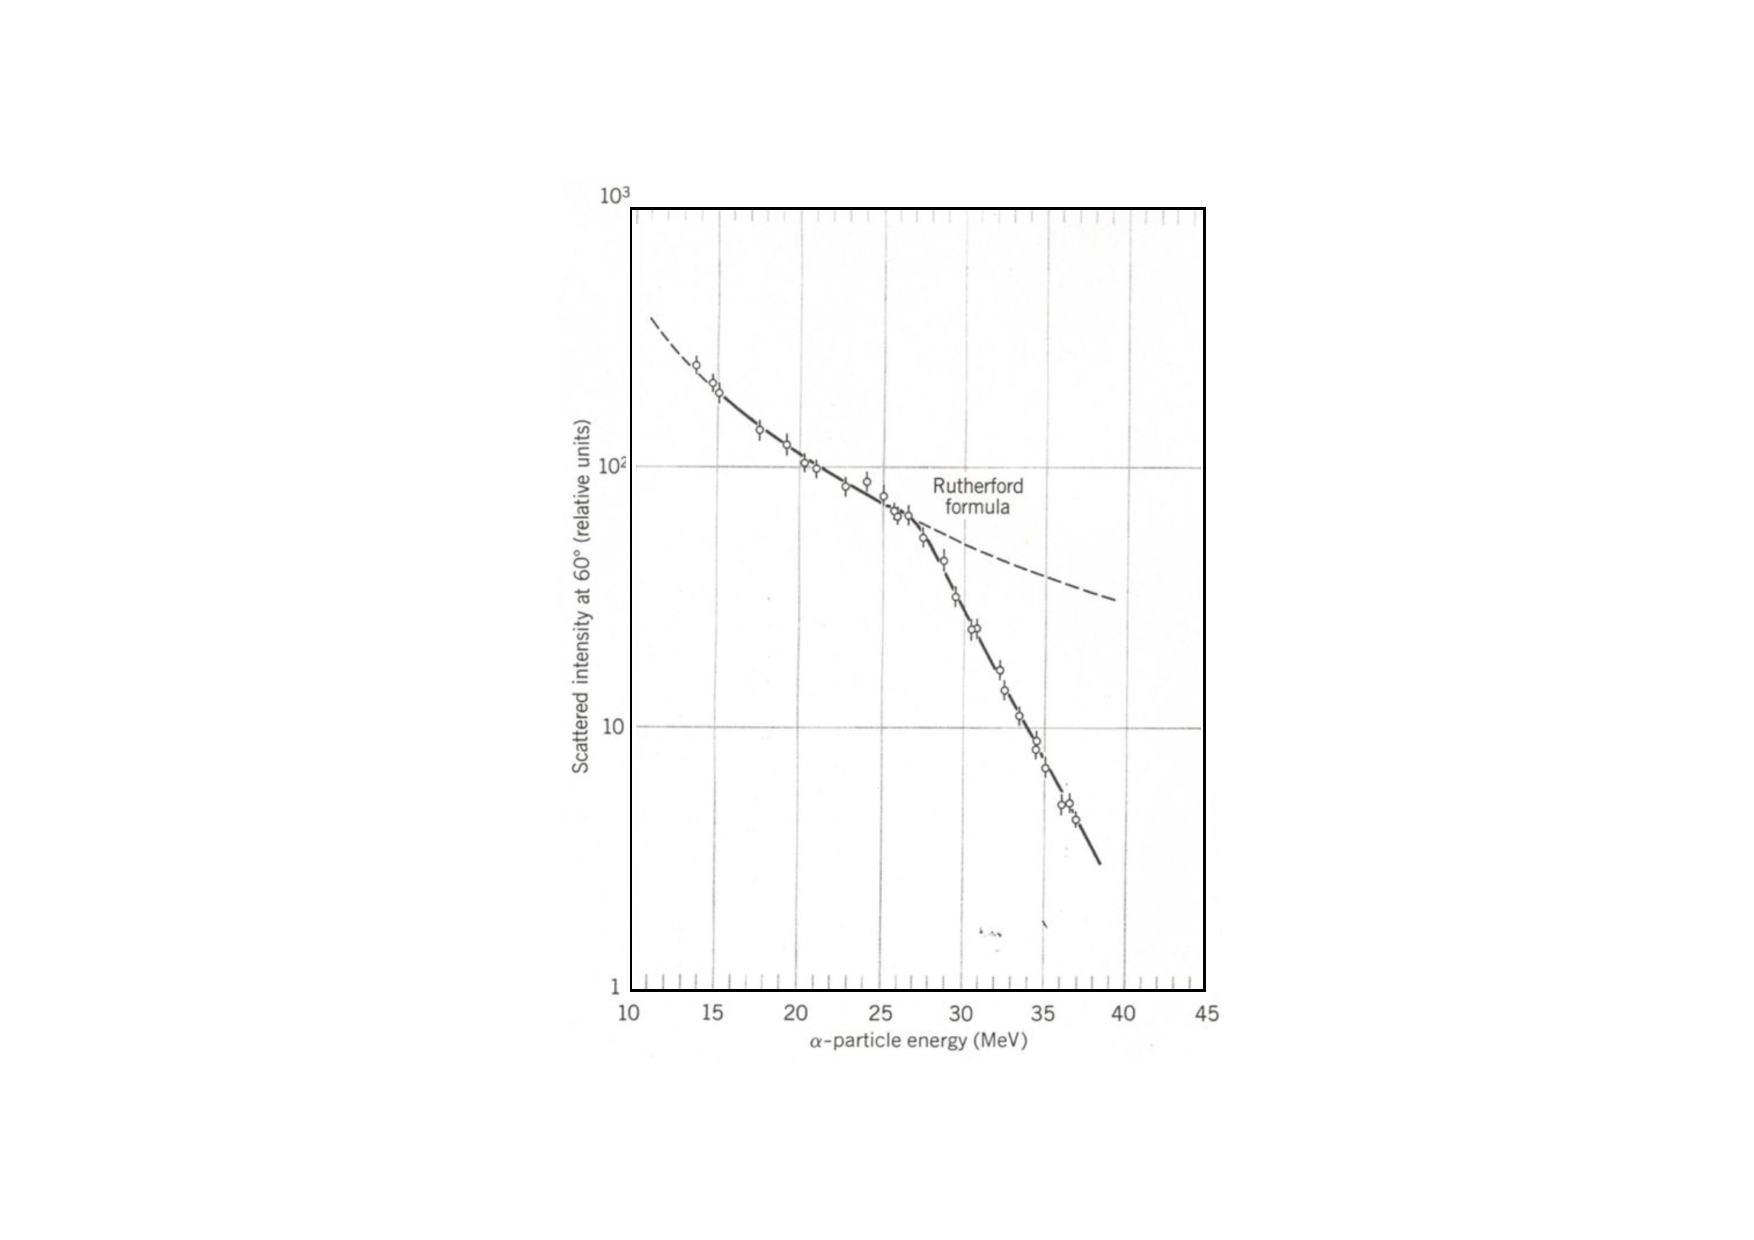
\includegraphics[width=0.65\textwidth]{R-Scattering}
    \caption{Measurement of the Rutherford cross section at a scattering angle of $\theta = 60^o$ with probe $\alpha$ particles with kinetic energy of up to approximately 40~MeV.}
    \label{fig:RutherfordScatteringBreakdown}
\end{figure}{}

These findings are crucial in building a theory of the interaction that holds the nucleus together, that will be referred to as the strong (nuclear) interaction -- as will be discussed in Chapter~\ref{chap:fundInteractions}. \\

Beyond giving a revolutionary picture of the atom (and now the nucleus), the formalism discussed in this section to derive the Rutherford formula will be used to discuss the interaction of particles in matter in Chapter~\ref{chap:InteractionsInMatter}.


\section*{Take-home lessons}
\begin{itemize}
    \item Scattering is an essential tool for studying the structure of molecules, atoms, nuclei and particles, and to study their properties and interactions. Scattering processes typically involve a particle being sent on a target, or two beams of particles scattering together.
    \item Elastic scattering is a scattering process in which the nature and number of the particles in the initial and final state are the same. Particles change only direction and energy, and the total kinetic energy is conserved.
    \item One basic concept for a quantitative description of scattering is that of \emph{impact parameter}. In classical scattering, for example when one rigid sphere undergoes elastic scattering with another sphere, impact parameter -- the distance between the centers of the two spheres -- fully determines the scattering angle (which is the angle at which the impinging sphere is deflected).
    \item In reality, scattering cannot be simply represented as the scattering of two rigid spheres. First of all, experiments typically involve a beam of particles colliding against some physical target, i.e. it's experimentally impossible to measure the motion of all single particles. Then, quantum mechanics states it's inherently impossible to know with arbitrary precision position and momentum of those particles. 
    \item In the case of a beam colliding over a fixed target, for example, one therefore needs to describe scattering by taking into account that the beam is composed by $N_A$ particles which travel its transverse surface $S$ with a flux $\phi_A=\od{N_A}{t}\frac{1}{S}$. The target is typically made of some physical material with $n_B$ target particles per unit of volume: if its length along the beam path is $d$, then the number of target particles seen by the beam is $N_B=n_b S d$.
    \item The ultimate question of scattering theory is: how many interactions $N_I$ between particles in the beam and particles in the target will happen in unit time, i.e. what is the scattering rate? In the case of a beam-target experiment, this rate is proportional to the flux of incoming particles and to the number of target particles seen by the beam, $\od{N_I}{t}=\sigma \phi_A N_B$. The proportionality factor $\sigma$ is called \emph{cross section}. Luminosity is instead defined as the product $\mathcal{L}=\phi_A N_B$.
    \item The cross section of a scattering process is a measure of the probability of that process to take place. Although cross section has the dimensions of the square of a length, it should not be interpreted as a measure of the relative physical size of the target with respect to the beam, like it is in the classical case of colliding rigid spheres.
    \item Luminosity is a property of the chosen experimental setup, not of the underlying interaction. One may in fact use different experimental setups -- for example, beam-target and beam-beam experiments -- to investigate the same scattering process. The interaction rate would then still be the product of cross section and luminosity.
    \item The density $n_B$ is the volume density of target particles in the physical target. Its role depends on which process one is considering: for example, in a scattering process between an electron beam and protons in a fixed, $n_B$ would be the number of protons in the atoms of the physical target, which can be expressed as a function of the atomic number, atomic mass and density of the target material.
    \item In real life one measures the position and energy of particles -- sometimes of all initial and final state particles, sometimes only of a few of them. Experiments are in general sensitive to \emph{differential} rates of interaction, which means that one measures how many particles are observed in unit time in a given portion of the solid angle, and/or how many of them have energy inside a given range. The differential interaction rate depends on the concept of differential cross section, which encloses the dependence of the interaction probability on quantities like the scattering angle and the particle energy. The integral of the differential cross section over those quantities gives of course the total cross section $\sigma$.
    \item How much a beam of particles can penetrate a fixed target is a function of the density of the target, and of the cross section of the interaction between beam and target particles. This process is inherently exponential, and is described by the absorption coefficient and its reciprocal, the attenuation length or mean free path.
    \item The Rutherford experiment proved that Thomson was wrong: atoms aren't uniformly filled with positive and negative charges, but rather they are made of small, positively-charged nuclei, around which negative electrons orbit. Rutherford sent a collimated beam of $\alpha$ particles on a thin gold target, and measured an interaction rate with a strong dependence on the scattering angle, compatible with the hypothesis of a sphere with a positive, small nucleus.
    \item The Rutherford experiment can be treated with a purely classical formalism, under the assumption that the $\alpha$ particle -- an helium nucleus -- undergoes an elastic scattering with the point-like gold nucleus, with which it interacts electromagnetically. The interaction potential which describes the interaction is therefore the Coulomb potential, which is central. The key to calculate  the differential interaction cross-section is finding the relation between the impact parameter and the scattering angle.
\end{itemize}
\section*{Questions}
\begin{itemize}
    \item What are the hypotheses which allow us to express impact parameter as a function of scattering angle, in Rutherford scattering?
    \item Are we really worried about the possible divergence of the Rutherford cross section at small angles?
    \item What would change in the Rutherford experiment if the atomic nucleus was negatively-charged? Can you think of a way to determine the charge of the nucleus?
\end{itemize}
